\chapter{Research Design}\label{chapter:survey_one}

The goal of this chapter is to document and describe the evaluation process of the Immotion warm up exergame in this thesis. The process is separated into three stages. In the first stage we assess the prototype of our gamified system and its elements. We evaluate through a survey which features of the gamified system are appreciated the most and which the least, and hence can be removed or improved. In the second stage, based on the feedback and reactions received from the respondents in the first stage, we complete the implementation of the second release of our gamified system. In the last stage, we pilot-test our gamified system in a local fitness center and evaluate it through a pilot-test study. In order to measure overall acceptance of our gamified solution for warm up, different methods have been used which will be described in the following sections.  The data is visualized using \textit{Tableau Desktop 10.3} software.

\section{First Evaluation}

The results from this evaluation should help to answer the overall research questions of this thesis:
\begin{enumerate}
\item \textit{Can exergames with gamification elements make warm up routines more enjoyable and, thus, motivate individuals to warm up more regularly before physically more demanding exercises?}
\item \textit{Can exergames with gamification elements be used as a interactive guidance for individuals who do not know how to perform warm up routines before physically more demanding exercises?}
\end{enumerate}

\section{Quantitative Methods}
To gain a first insight into acceptance of the Immotion warm up game we created an online survey. The survey was created using \textit{Google forms} and was accessible for two weeks from 16th to 30th of July 2017. The survey has been advertised via social networking services (\textit{Facebook} and \textit{LinkedIn}) and e-mail lists. No incentives were used to collect responds for this survey. Since our gamified system ought to be used before physically more demanding exercise (training) in gyms, fitness and sports centers, we targeted individuals who are physically active and engage in some sort of physical (sport) activity on a regular or semi-regular basis. The goal of this survey was to explore general work out and warm up habits of the respondents and their preferences and general acceptance of a gamified solution of a warm up routine. The questions in the survey were divided into three parts. First, the participants were asked a set of general questions regarding their age, gender and education level. Next, their training habits and warm up preferences were assessed. Lastly, participants were showed a video of the prototype version of the warm up game and asked questions related to the presented gamified warm up solution. 

\subsection{General Questions}
In the first part of the survey, the respondents are asked general questions about their gender, age and education level. Total number of n = 446 individuals participated in the survey, of which n = 204 (45.7\%) were female and n = 242 (54.3\%) male. The age of the respondents ranged from 17 to 58 with an average age of 30.16 years (SD = 6.49). The  following trend chart in \ref{fig:AgeTrend} shows the number of respondents grouped by their age.\\
\begin{figure}[h]
    \centering
    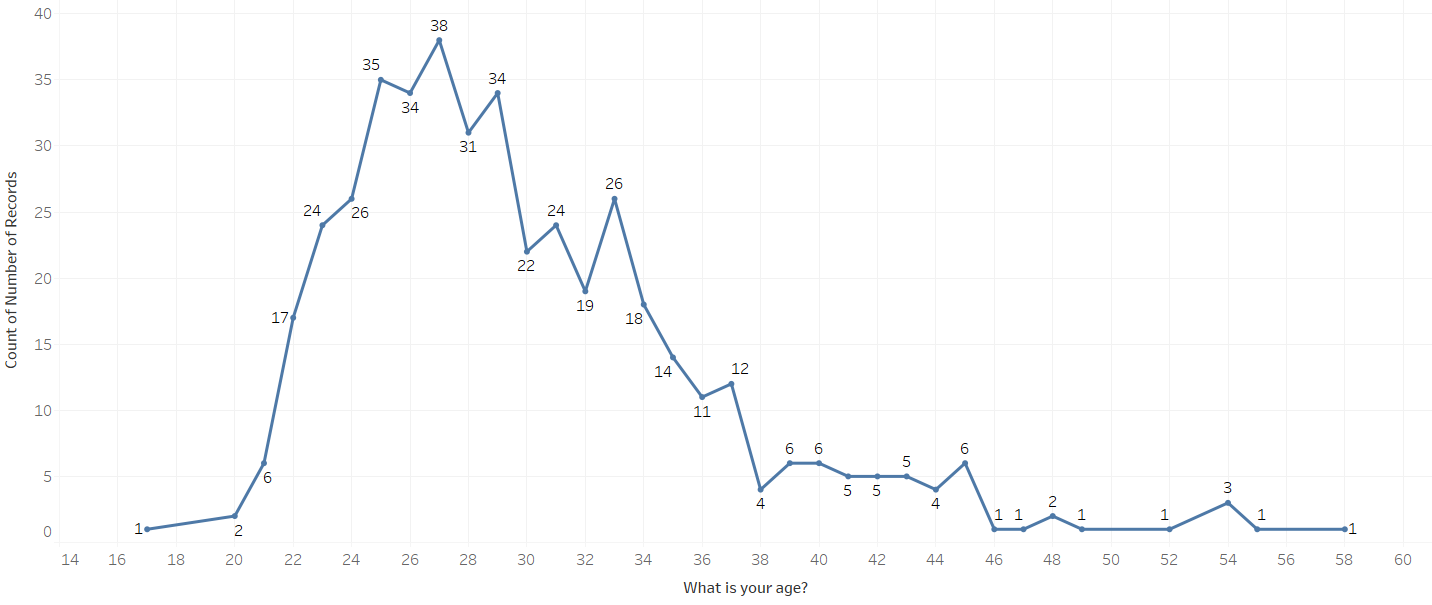
\includegraphics[width=\textwidth]{AgeTrend}
    \caption{The trend chart of respondents' age}
    \label{fig:AgeTrend}
\end{figure}\\
We observe that the most number of the survey participants are between 22 and 35 years old.\\
Regarding participants' education level, the majority of the respondents completed either their Master's studies n = 209 (46.9\%) or Bachelor studies n = 151 (33.9\%). The pie chart in \ref{fig:Education} shows the number of respondents based on their education level. 
\begin{figure}[h]
    \centering
    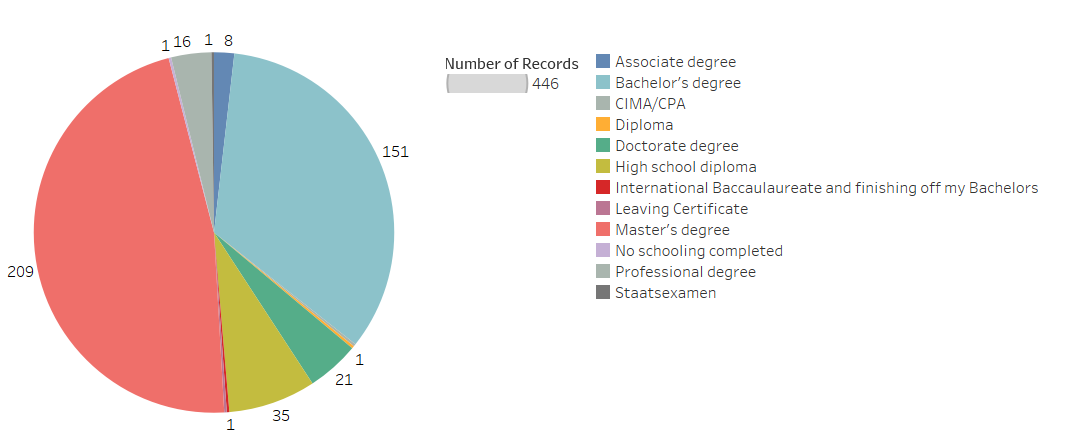
\includegraphics[width=\textwidth]{Education}
    \caption{Respondents' education level}
    \label{fig:Education}
\end{figure}
\subsection{Questions Related to Work Out and Warm Up Preferences}
The second section of the survey evaluated the respondents work out and warm up preferences. Total number of n = 442 of the respondents were amateur (recreational) athletes (99.1\%), while only n = 4 individuals declared themselves as being a professional athlete. In the survey, the respondents were pointed out that the most basic difference between amateur and professional athletes lies in the rewards that each group receives for athletic performances. Generally speaking, amateur athletes are not paid for their athletics performances. Professional athletes, by contrast, are typically paid annual salaries plus incentives tied to individual and team performance \cite{amateurvsproffesional}. More than half of the respondents (n = 357) reported taking part in some sort of sports activities during the whole year (77.4\%), while n = 101 (22.6\%) only few months per year. This means that most of the respondents engage in physical activities regularly without any longer stoppage.\\Regarding weekly training session occurrences, n = 152 respondents reported having 1 to 2 (34.1\%) and n = 168 having 3 to 4 (37.7\%) work out or sports sessions per week, while n = 54 (12.1\%) respondents reported taking part in sports activities irregularly (less than once per week). Most of the respondents (n = 285) reported having training sessions which last between 1 and 2 hours (63.9\%). The second most prominent training session duration reported by n = 125 respondents was less than an hour (28\%). Only n = 35 respondents reported having sport session with duration more than 3 hours. In \ref{fig:wuPreferences}, the pie chart on the left shows the percentage of respondents based on the number of training sessions per week. The pie chart on the right shows the percentage of respondents based on the duration of their training session. Moreover, n = 251 respondents stated that they prefer exercising alone (56.3\%), n = 86 (19.3\%) with a friend (or friends) and n = 109 in a group (24.4\%). Having a personal trainer was not prevalent among the respondents, and only n = 52 reported exercising with a personal trainer. 
\begin{figure}[h]
    \centering
    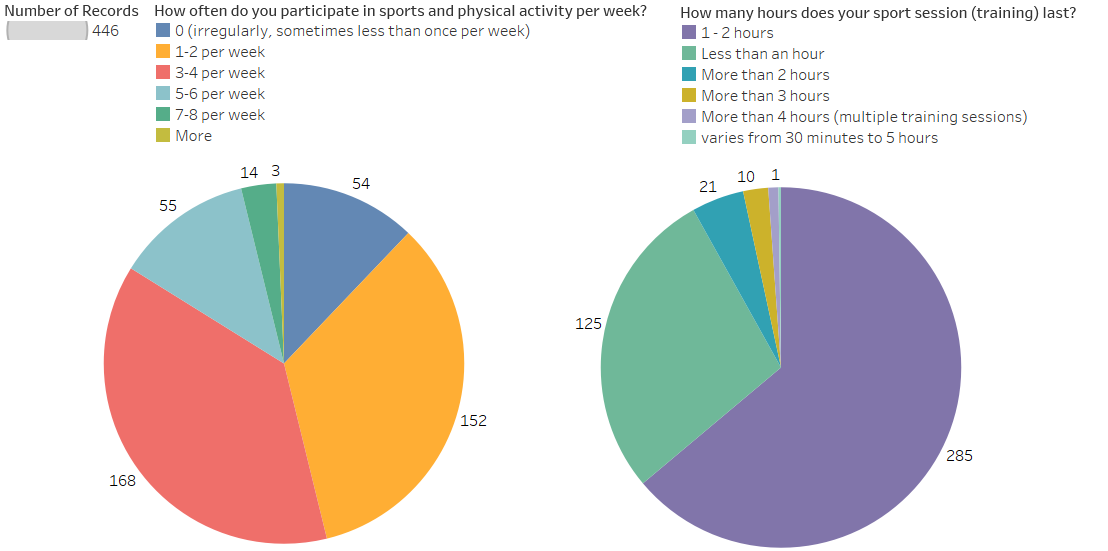
\includegraphics[width=0.80\textwidth]{wuPreferences}
    \caption{Respondents' weekly training session number and training duration}
    \label{fig:wuPreferences}
\end{figure}\\
When asked about their warm up preferences before a physical activity, n = 251 respondents (56.3\%) reported always warming up before physically more demanding exercises (or sports activities), whereas n = 195 (43.7\%) reported not warming up regularly before physically more demanding exercises (or sports activities). These results additionally confirm our assumption regarding absence of warm up habits in multitude of athletes. In \ref{fig:wuHabits}, we represent the respondents' warm up habits with regard their preferences to exercise alone, in a group or with a friend. 
\begin{figure}[h]
    \centering
    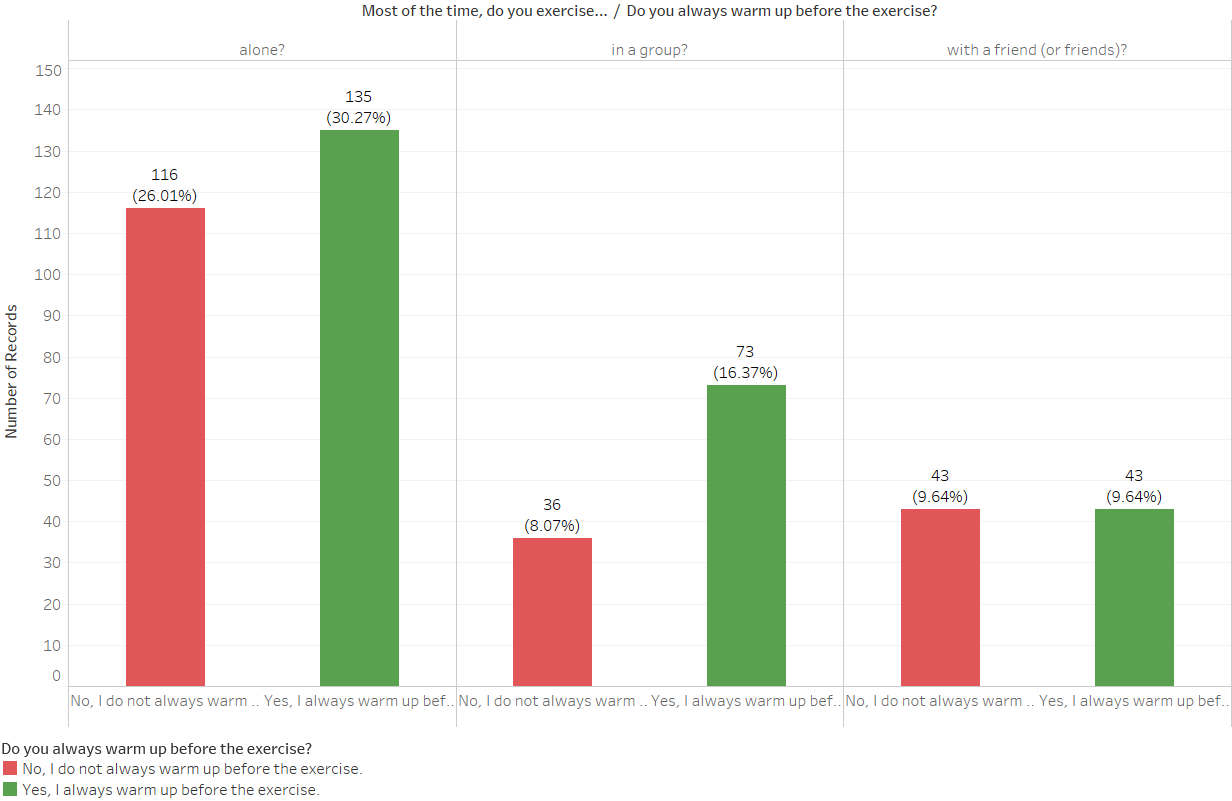
\includegraphics[width=0.80\textwidth]{wuHabits}
    \caption{Sum of Number of Records for the question ``\textit{Do you always warm up before the exercise?}'' broken down by ``\textit{Most of the time, do you exercise alone/with a friend/in a group?}'' Color shows details about ``\textit{Do you always warm up before the exercise?}''}
    \label{fig:wuHabits}
\end{figure}\\
It is interesting to notice that the most number of respondents who stated not warming up regularly, reported preferring exercise sessions that are carried out alone. On the other hand, we notice that most individuals who reported exercising in a group, regularly warm up before some sports activity. Based on their answer regarding warm up preferences, respondents were further asked different set of questions. Respondents that have stated not warming regularly, have been asked about reasons for not doing so. On the other hand, respondents who reported warming up regularly have been inquired about the duration and types of warm up exercises they usually engage in.
\subsection{Questions Related to Warm Up Routines}
The pie chart in \ref{fig:wuDuration} shows the number of respondents based on the duration of their warm up sessions before physically more demanding exercise. Only those respondents who reported warming up regularly were asked this question. Among n = 251 respondents that reported always warming up before the training session, the most common duration was between 5 and 10 minutes (43.4\%). Next, n = 66 (26.3\%) reported warming up less than 5 minutes, n = 64 respondents (25.5\%) between 5 and 10 minutes and, lastly n =11 (4.4\%) reported warming up more than 15 minutes. Only one respondent reported warming up less than a minute. The answers related to warm up duration gathered from respondents gave us valuable information about the most prevailing duration of warm up sessions. By knowing this, we can limit the duration of our warm up game to correspond to the periods outlined by the respondents through the survey.   
\begin{figure}[h]
    \centering
    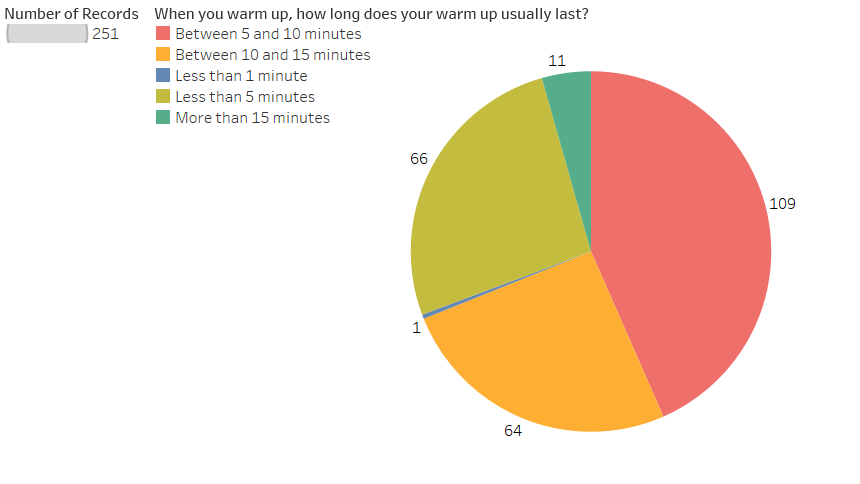
\includegraphics[width=0.90\textwidth]{wuDuration}
    \caption{ Responds to the question ``\textit{When you warm up, how long does your warm up usually last?}''}
    \label{fig:wuDuration}
\end{figure}\\
When the reported duration of the training session and warm up are compared among the respondents who stated warming up before the physically more demanding exercise, it is evident that the most common warm up duration is between 5 and 10 minutes regardless of the training session duration. In case of training sessions with duration less than 1 hour, the second most common warm up duration is the one that is less than 5 minutes long. On the other hand, in case of training sessions with duration between 1 and 2 hours, the second most common warm up duration is between 10 and 15 minutes. The highest number of respondents who stated warming up between 10 and 15 minutes belong to the group with the training session duration between 1 and 2 hours. In this group, less than 5 minutes warm up sessions were also customary. Overall, we can conclude that individuals do not tend to spend less than 1 and more than 15 minutes on the warming up procedure before physically more demanding exercises. The results are shown in \ref{fig:wuDuration2}.\\
\begin{figure}[h]
    \centering
    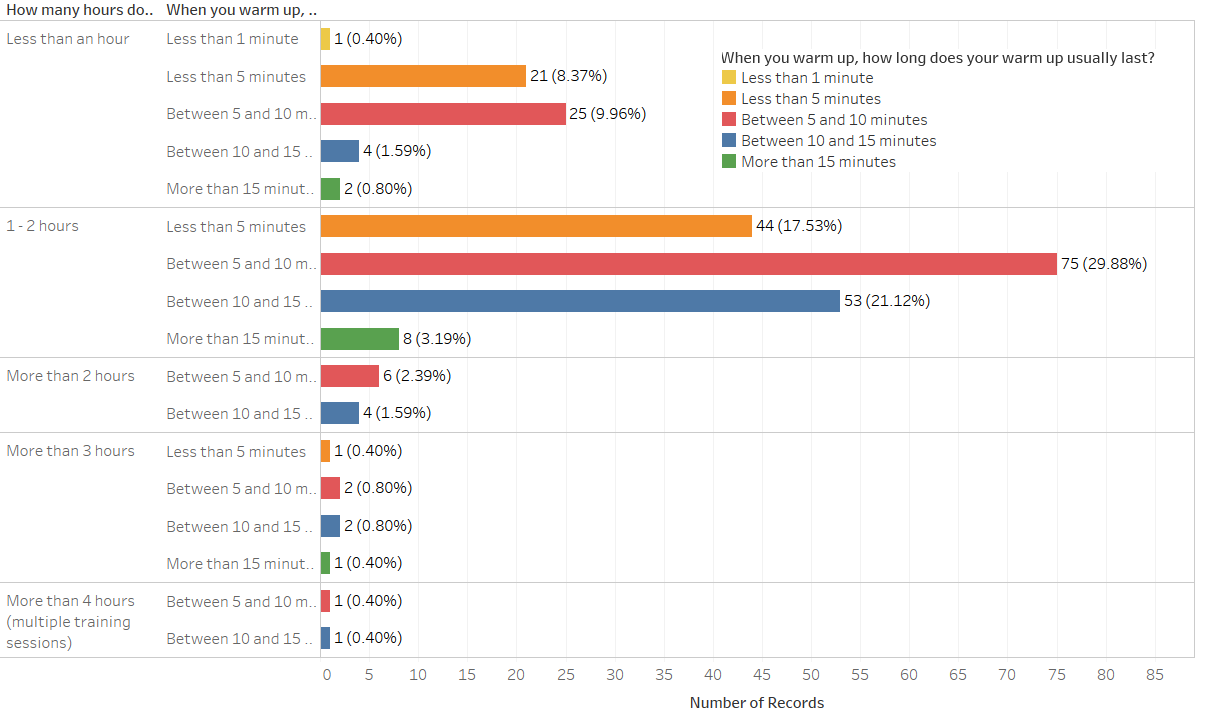
\includegraphics[width=\textwidth]{wuDuration2}
    \caption{Sum of Number of Records for each ``\textit{How many hours does your sport session (training) last?}''. Color shows details about ``\textit{When you warm up, how long does your warm up usually last?}''}
    \label{fig:wuDuration2}
\end{figure}\\
Taking this into account, the second release of the Immotion warm up game will enable players to choose the warm up duration they prefer the most. The available duration to choose from will be 1 minute, 2 minutes, 3 minutes, 5 minutes, 7 minutes, 10 minutes and 15 minutes which aligns to the duration pointed out by the respondents. These durations align also with the most common ones outlined in Chapter \ref{chapter:relatedwork} and suggested by different sources \cite{bishop2003warm2}.\\\\\\Respondents who reported warming up regularly were also inquired about the type of the warm up exercises they perform before the sport activity. Respondents could choose among three warm up types most often referred to in sports literature \cite{shellock1985warming, bishop2003warm2}, which were: 
\begin{itemize}
\item general warm up,
\item sport specific warm up (warm up that reflects the type of movements and actions which will be required during the sporting event), and 
\item passive warm up (e.g., taking a hot shower, having a rubdown, sitting in the sun)
\end{itemize} As mentioned, this question was asked only from those respondents that reported always warming up before the sport activity (n = 251). The most common warm up routine, reported by n = 140 respondents (55.8\%), was the sport specific type while the general (non-specific) warm up type was reported by n = 111 (44.2\%) of them. None of the respondents reported performing passive warm up before the more demanding physical activity. While using the Immotion warm up game, the player is asked to perform a set of general warm up exercises in order to complete the game. Hence, it was necessary investigate athletes preferences towards types of warm up routines they engage in most often. More than half of the respondents (55.8\%) reported engaging in sport specific warm up routine. This indicates that the respondents are more inclined towards specialized and personalized warm up routines, as opposed to the ones required in the prototype warm up game. Thus, the game should support players in selecting the set of warm up routines that are less general and more sport specific based on the sport they want to play (or group of muscles they want to warm up) or diversify and increase the types of movements the player needs to perform in order to successfully finish the game. %we believe that if the number and the type of movements are increased...%
Furthermore, n = 140 (55.8\%) respondents out of n = 251 reported having no inclination towards warming up in a group. Also, n = 101 (40.24\%) respondents stated not following any warm up procedure. Next, when asked about their preferences towards warming up when given instructions, n = 156 (61.4\%) out of n = 251 reported favoring warm up sessions when they are instructed and demonstrated by someone else. This is a valuable information because it suggests that individuals could, presumably, be inclined to warm up more regularly if they had a guidance through the warm up routine. With the Immotion game, we tackle exactly this requirement. By placing the obstacles that are to be avoided and coins to be collected, the athlete is instructed and guided through the warm up routine from the moment the game begins.\\The Immotion warm up game is designed and implemented as a single player game that guides the players through the warming up process and instructs them to perform specific movements in order to finish the game successfully and, consequently, warm up major muscle groups. Hence, it was required to assess these warm up preferences. In addition, out of n = 251 respondents, n = 111 (44.2\%) reported enjoying warm up sessions when they are carried out in a group. This leads us to believe that multiplayer (group) warm up should also be an option in the Immotion warm up game. That way, both athlete types (the ones preferring warming up individually and the ones not) can utilize and benefit from the game. Lastly, n = 150 respondents (59.76\%) stated following some warm up procedure. This result was unanticipated. However, it suggests that most of the athletes who took the survey and do warm up regularly, are well aware of the beneficial effects of warm up routines, and by following well established and accepted ones, are trying to maximize its positive outcomes. In \ref{fig:wuPrefPie}, the pie chart on the left shows the percentage of respondents who prefer warming up when given instructions (and those who do not), the pie chart in the middle shows the percentage of respondents who follow some recommended warm up procedure (and those who do not) in a group and those who do not and, lastly, the pie chart on the right shows the percentage of respondents who prefer warming up in a group (and those who do not).
\begin{figure}[h]
    \centering
    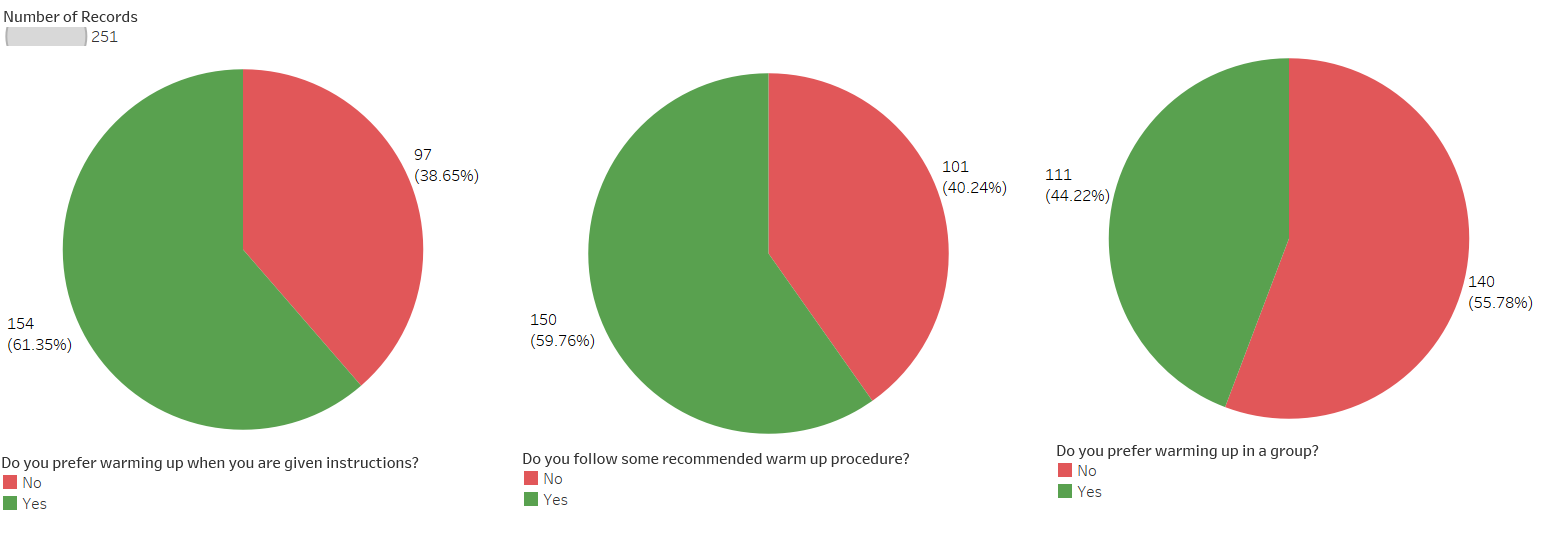
\includegraphics[width=\textwidth]{wuPrefPie}
    \caption{Respondents' answers for question ``\textit{Do you prefer warming up when you are given instructions}'', ``\textit{Do you follow some recommended warm up procedure}'', ``\textit{Do you prefer warming up in a group}''}
    \label{fig:wuPrefPie}
\end{figure}\\
The pie chart in \ref{fig:wuIntroduce} shows the number and percentage of respondents based on their answer on the question ``\textit{How were you introduced or recommended to the warm up procedure?}''.
\begin{figure}[h]
    \centering
    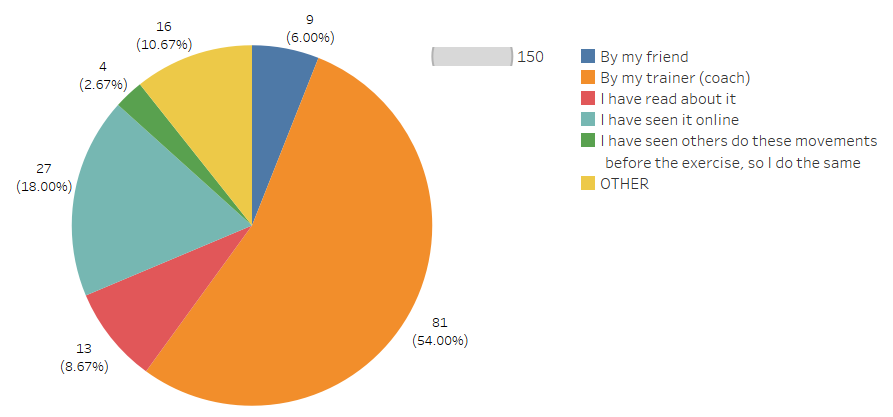
\includegraphics[width=\textwidth]{wuIntroduce}
    \caption{Sum of Number of Records and Percentage of Total Number of Records for the question ``\textit{How were you introduced or recommended to the warm up procedure?}''}
    \label{fig:wuIntroduce}
\end{figure}\\
Answering this question was optional, and it was asked only from those respondents who reported warming up regularly. Among n = 150 respondents that gave answer to this question, n = 81 (54\%) stated that they were introduced to the warm up procedure they perform by their coach, n = 27 (18\%) have seen the procedure online, while n = 13 (8.67\%) have read about it. The rest of the respondents reported seeing others do similar movements before the sports activity (n = 4) and to be introduced to the warm up procedure by their friend (n = 9). Some of the other sources, reported by n = 16 respondents were:
\begin{itemize}
\item ``\textit{I am a certified personal trainer, so I've adapted my learning to my own training}''
\item  ``\textit{Exercise APPs}''
\item  ``\textit{Physio + Personal trainers + coaches + YouTube channels}''
\item  ``\textit{Studied as part of college course}''
\end{itemize}
To assess respondents' attitude towards the importance of the warm up procedure before physically more demanding exercise, the respondents (n = 251) were asked to give their preferences regarding the following statements: 
\begin{itemize}
\item ``\textit{Warm up before exercise is important for me.}''
\item  ``\textit{Warm up before exercise can positively affect my performance.}''
\item  ``\textit{Warm up before exercise can reduce the likelihood of an injury.}''
\item  ``\textit{After my warm up routine, I feel I am prepared for the physically more demanding activity.}''
\end{itemize}
For each question, respondents could choose among five categories: \textit{Strongly Disagree}, \textit{Disagree}, \textit{Neutral}, \textit{Agree} and \textit{Strongly agree}. Each category is assigned a score from 1 (Strongly Disagree) to 5 (Strongly Agree). In \ref{fig:LS1} we show the  
\textit{Likert} scale score for the previous statements broken down by respondents' gender. For each question we assign a range of values that show how the survey responses are spread by category and a general feeling whether they are positive or negative. Based on the available categories and their total scores, we specify the dividing line and check how many responses are below and above it. That is, the dividing line is at 0\% and the responses left from it are generally negative, and right from it generally positive.  Each individual line shows a different starting point for each answer. The offset (lines' starting point) depends on the total number of negative scores, which are in our case the number of Neutral, Disagree and Strongly Disagree divided by the overall score for that question. The overall score (or the number of responses) for all the question is the same, since these questions were mandatory and all respondents answered it. Also, we split the Neutral answers and assign half of it to positive, and half to negative answers so we are not weighting unfairly one side to the other.  The width of each individual category depends on the number of records that are in that category over the total number of responses for the entire bar (that particular question). Lastly, we add the overall Likert scale score depicted as a yellow circle in each bar which shows the summary for each individual question.  
\begin{figure}[h]
    \centering
    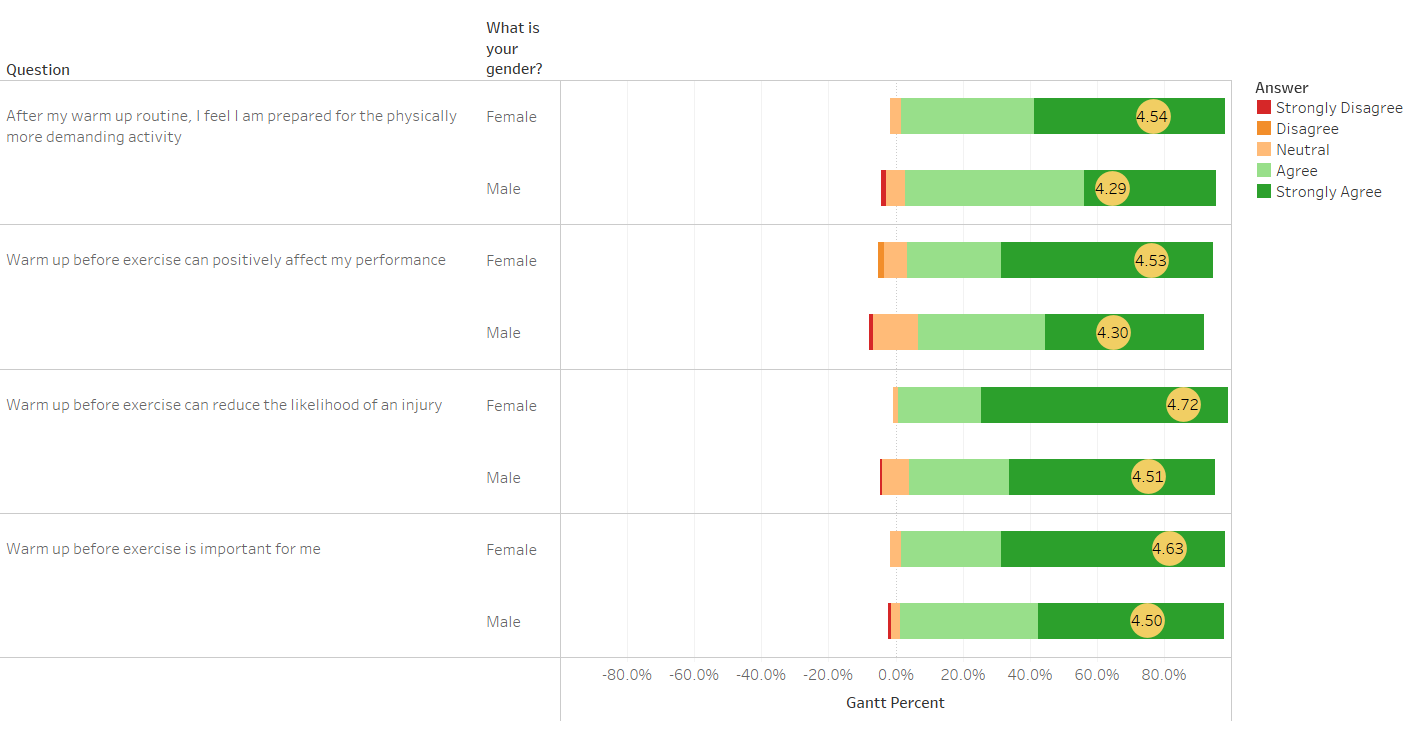
\includegraphics[width=\textwidth]{LS1}
    \caption{Gantt Percentage and the average score for the following statements: ``\textit{Warm up before exercise is important for me.}'', ``\textit{Warm up before exercise can positively affect my performance.}'', ``\textit{Warm up before exercise can reduce the likelihood of an injury.}'', ``\textit{After my warm up routine, I feel I am prepared for the physically more demanding activity broken down by respondents gender.}''}
    \label{fig:LS1}
\end{figure}\\
From the responses that are presented in \ref{fig:LS1}, we conclude that the respondents have a generally positive stand towards the statements given, since every question has an overall Likert score above 4 out of maximum 5. This positive bias was somewhat expected since the question was asked only from those who reported warming up regularly before sports activities. Some lower scores were obtained for male respondents in the first two statements ``\textit{After my warm up routine, I feel I am prepared for the physically more demanding activity}'' (4.29) and ``\textit{Warm up before exercise can positively affect my performance}'' (4.30) which might indicate that a number of the respondents, even though warming up regularly, do not perform the warm up procedure thoroughly and thus, do not feel fully prepared for the subsequent sports activity.\\ Respondents who stated warming up regularly were asked to describe their warm up routine or to list the most common exercises they perform in order to prepare for the physically more demanding ones. Since  n = 150 respondents (59.76\%) stated following some specific and well established warm up routines, we were interested in the most common movements and exercises these routines combine. Our primary goal was to use those movements and exercises in the game as movements for avoiding obstacles and collecting points. After the answers are collected, we group them based on textual occurrences of specific keywords and on textual occurrences of keywords with the same semantic meaning. The aggregated answers are shown in \ref{fig:5_describeWURoutine}.
\begin{figure}[h]
    \centering
    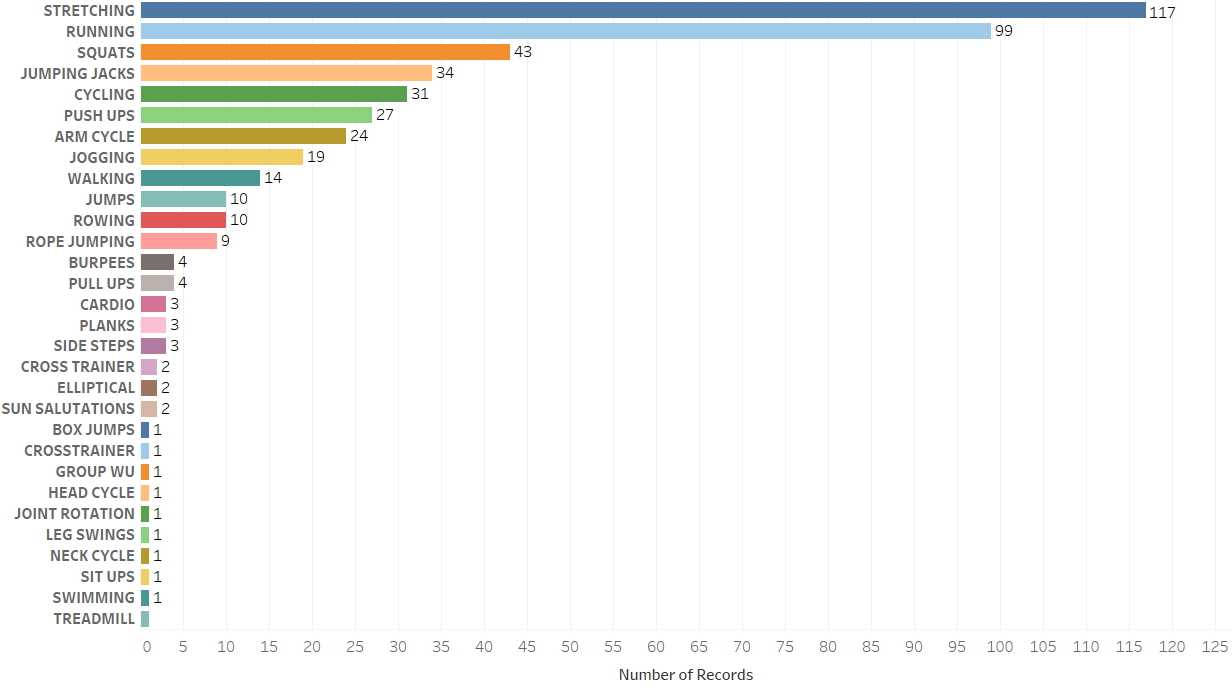
\includegraphics[width=\textwidth]{5_describeWURoutine}
    \caption{Summary of most common warm up exercises performed by the respondents}
    \label{fig:5_describeWURoutine}
\end{figure}\\
From \ref{fig:5_describeWURoutine}, we observe that the most of the respondents include stretching exercises in their warm up routine. This was expected since, when asked if they include stretching in their warm up procedure, out of n = 251 respondents, n = 205 reported performing, while n = 46 reported not performing stretching exercises during warm up session. We hypothesize that the reasons for this is that athletes confuse stretching with warming up and believe stretching exercises can prepare our body for strenuous activity as well as prevent injuries. However, as already pointed out in Chapter \ref{chapter:relatedwork}, there exists no scientific evidence for these assumptions. Additionally, in a recent study that included 2729 runners, static stretching had proved to have no effects in protecting against injury. According to the researchers, "stretching neither prevented nor induced injury when compared with not stretching before running" \cite{pereles2012large}. In some cases, a study published in Medicine and Science in Sports and Exercise (PubMed) found, it can even inhibit performance. After reviewing the available literature, the authors point out that static muscle stretches which are longer than 60 seconds are more likely to lead to a slight to moderate reduction in performance \cite{kay2012effect}. Hence, we believe that, by using our gamified solution, not only that athletes can prepare themselves for the subsequent physical exercises but also be more informed about the most efficient and practical movements that presumably reduce the likelihood for injuries and increase body performance for the subsequent physical activity. The second most common exercise is running (indoor and outdoor). The respondents usually start their warm up with a few minutes run after which they perform a full body stretching exercises. Apart from that, exercises like squats, jumping jacks, push-ups, arm cycles and cycling are also common exercises among the respondents. Some respondents, on the other hand, use treadmill, cross trainer, rowing and elliptical exercise machine for warming up. From the answers, we can conclude that respondents mostly focus on warming up their lower body parts in their warm up routines and in general finish the warm up routine with whole body stretching exercises. We also notice that most of the respondents do not follow any specific warm up routines and use general exercises before sports activities with strong focus on whole body stretching.\\Certain number of respondents, on the other hand, did not only list but described an exemplary warm up routine. Some of them are: 
\begin{itemize}
\item ``\textit{Warm up depends on exercise: e.g. warming up for heavy squats includes hip-opening exercises, core static exercises, mobility exercises for hip rotation/extension, low-weight squats.}''
\item ``\textit{For climbing: running on the spot, arm cycles, ankle rotations, active and passive stretches of leg, arm and back muscles.  For running: running on the spot, ankle rotations, active and passive stretches of leg muscles}''
\item ``\textit{I start with an activity to raise my heart rate and body temperature. Once that's accomplished, I work through stretching the major muscle groups first, then typically sit down to stretch out smaller/more specific muscle groups.}''
\end{itemize}
Based on these answers we introduce new movements for avoiding obstacles and collecting points in our second release of the warm up game. As for the respondents, our main focus are lower body parts. Even though it is expected by the respondents, stretching exercises will not be incorporated. However, we inform the athletes after the game ends about the most preferred stretching duration they can perform in order to maximize the subsequent performance and, possibly, avoid injuries. Since we are using only one Kinect device for gesture tracking, we avoid complicated movements that require prior exercise knowledge or experience and increased focus. Moreover, taking into account our hardware constraint, we choose movements that are easily detectable with only one Kinect sensor. 
\subsection{Reasons for Not Warming Up}
Respondents who reported not warming up regularly have been inquired about the reasons for not doing it.  Out of n = 195 respondents who reported not warming up regularly before sports activities, total of n = 321 responses have been collected, since some of the respondents gave multiple answers to this question. The most common reasons reported by the respondents were time constraint which was reported by n = 84 respondents and the monotonous and tiresome nature of the warm up procedure, reported by n = 81 respondents. Furthermore, n = 41 respondents pointed out that the reason for not warming up was because they do not know how to properly carry out the warm up procedure, while for n = 37 respondents stated that the warm up procedure represents an insignificant and negligible activity. Figure in \ref{fig:Reasons} shows the respondents' answers regarding reasons for skipping warm up exercises before physically more demanding exercises.
\begin{figure}[h]
    \centering
    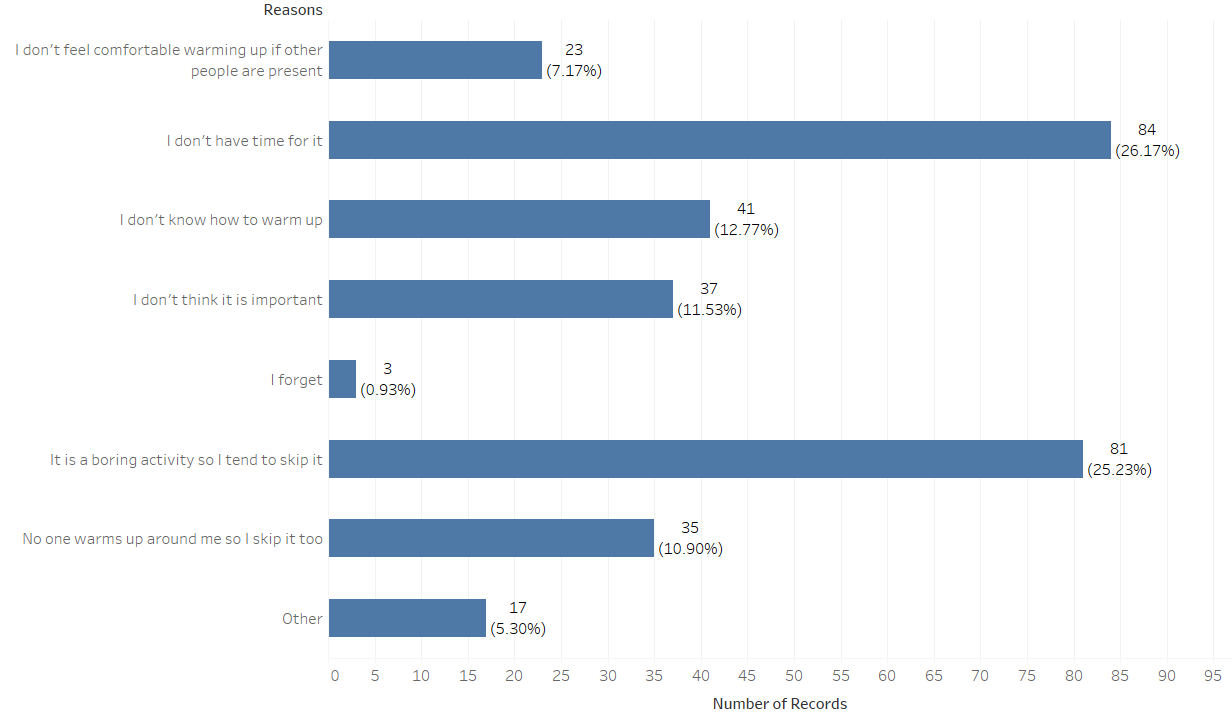
\includegraphics[width=\textwidth]{Reasons}
    \caption{Sum of Number of Records for respondents' reason for not warming up.}
    \label{fig:Reasons}
\end{figure}\\
Since this was an open ended question, a number of respondents left a comment regarding reasons for not warming up. We group all these answers in the Other category. Some of the other reasons for avoiding warming up pointed out by n = 17 respondents were: 
\begin{itemize}
\item ``\textit{I train climbing, so sometimes I can't wait to start climbing and skip the warm up.}''
 \item ``\textit{When I bike (for commuting) or do yoga, I don't warm up before, as I don't find it necessary.}''
\item ``\textit{I do a lot of endurance sports like running or biking. Warming up is kind of built in. If I do intervals, I do warm up.}''
\item ``\textit{It depends on the type of exercises - if I'm going for a bicycle ride I will skip warm up.}''
\item ``\textit{I feel it is better for me to warm up by playing the game.}''
\item ``\textit{It is part of the exercise. I dance, so the warm up is a dance routine.}''
\end{itemize}
We conclude that the reasons for not warming up are mostly tied to the specifics of the sports the respondents engage in. That is, these respondents believe that warm up for sports like biking, climbing or dancing are part of the exercise and they do not find it necessary to spend time for additional exercises that can prepare them for physically more demanding ones.\\In \ref{fig:ReasonsMaleFemale} we present the respondents' answers regarding reasons for skipping warm up exercises before physically more demanding exercises broken down by their gender.
\begin{figure}[h]
    \centering
    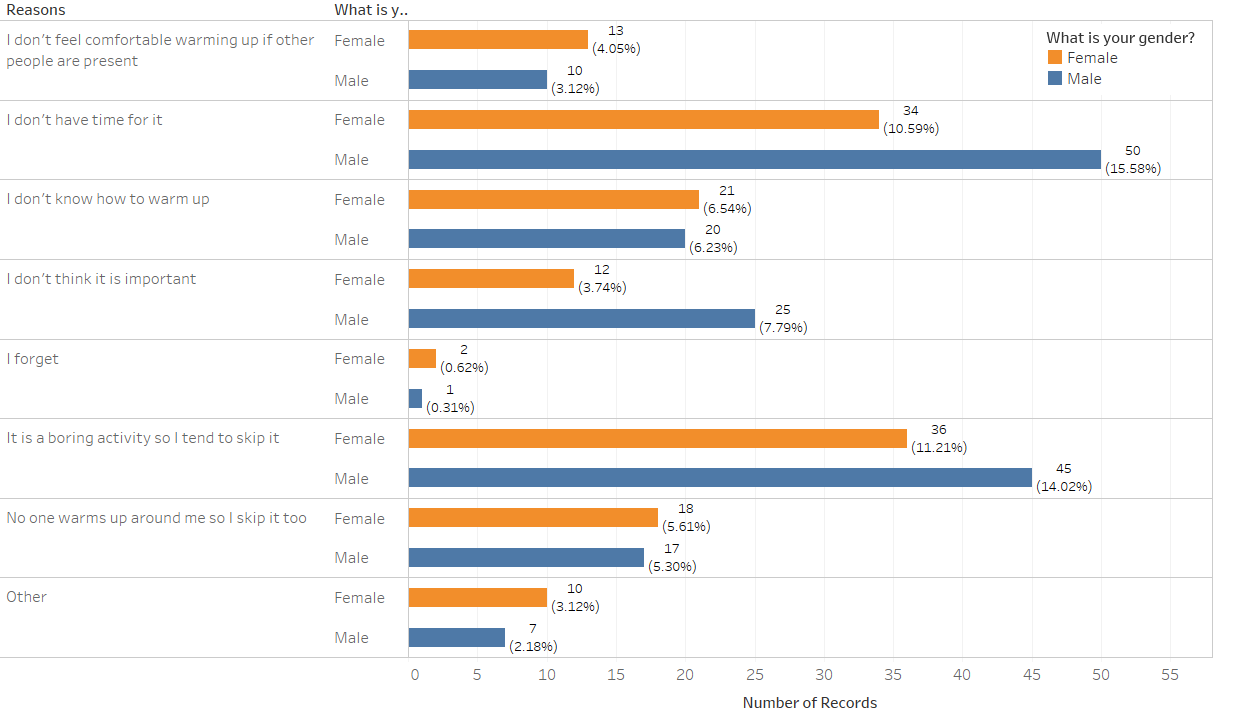
\includegraphics[width=\textwidth]{ReasonsMaleFemale}
    \caption{Sum of Number of Records for respondents' reasons for not warming up sliced by respondents' gender.}
    \label{fig:ReasonsMaleFemale}
\end{figure}\\
From the responses depicted in \ref{fig:ReasonsMaleFemale}, we observe that there were more male respondents that reported time constraints, dullness and meaningless of the warming up procedure as main reasons for not warming up before sports activities. On the other hand, more female respondents reported not feeling comfortable warming up when other people are present, not knowing how to perform the warm up procedure and avoiding warm up exercises because no one is doing it as main reasons for not warming up before sports activities. \\Next, in \ref{fig:ReasonsDoYouExercise} we present the respondents' answers regarding reasons for skipping warm up routine before physically more demanding exercise separated by their preferences toward warming up alone, with a friend or in a group. We notice that the most number of respondents who reported not warming up due to time constraints (n= 51), monotonous (n = 47) and, for them, meaningless nature (n = 25) of the warm up procedure usually engage in sports activities alone. 
\begin{figure}[h]
    \centering
    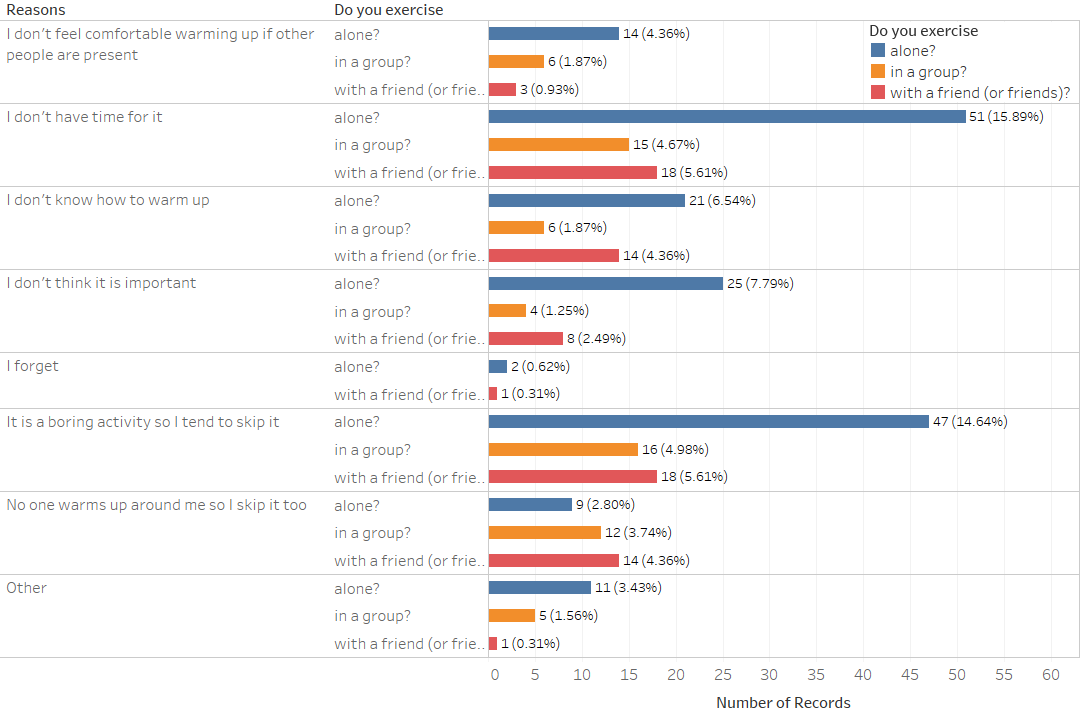
\includegraphics[width=\textwidth]{ReasonsDoYouExercise}
    \caption{Sum of Number of Records for respondents' reasons for not warming up sliced by respondents' work out preferences.}
    \label{fig:ReasonsDoYouExercise}
\end{figure}
Moreover, we observe that individuals tend to skip warm up more in cases when no one warms up in the group they are part of. That is, respondents who reported preferring sports activities which are carried out in a group or with a friend are likely to skip the warm up procedure if no one in the group engages in the warm up routine. In addition, this was the only case where a reason for not engaging in warm up had more responses in a category of respondents that usually work out with a friend or in a group. For all other reasons, most of the respondents belong to a category in which individuals reported engaging in sports activity usually alone. Hence, we conclude that individuals who carry out a sports activity alone, are more likely to skip the warm up routine than the ones doing it with a friend or in a group.\\ Overall, the results obtained in this question align with the ones acquired by Fradkin, \textit{et al.} (2010) in their survey on golfers and their warm up habits \cite{fradkin2010effects}. This further confirms the assumption addressed in this thesis and justifies the need for a solution that will motivate athletes to warm up more regularly before sports activities. Considering all the physiological and psychological benefits of a proper warm up routine and its suggested role in injury prevention covered in Chapter  \ref{chapter:relatedwork}, it is still perceived as a tiresome and meaningless activity and hence avoided by many amateur and professional athletes. Thus, educational and motivational solutions, that are enjoyable and easy to carry out, with primary focus on the major muscle groups and benefits of warm up need to be developed and implemented in order to increase the proportion of athletes who engage in warm up routines before every strenuous exercise.\\
With the Immotion warm up game, we tackle these issues brought up by the respondents. Making the game interactive and appealing, with intervals that last as long as the player chooses to, the warming up procedure undergoes a shift from a repetitive and tiresome activity to an entertaining and challenging necessity. Time constraints, mentioned by n = 34 female and n = 50 male respondents, will not be prevalent, since the player can choose the duration of the warm up session and by doing so plan ahead the work out session. These values are derived from the most common warm up duration reported by the respondents in \ref{fig:wuDuration}. Furthermore, athletes who do not know how to warm up and which movements to perform (mentioned by n = 21 female and n = 20 male respondents) in order to prepare their body for the subsequent sports activity, will be instructed through the game to perform a set a general warm up exercises. We believe that the guidance offered in our exergame could make the warm up routine more inviting for athletes who most often avoid or do not know how to perform the warm up routine properly. Moreover, we hypothesize that, if the athletes are provided with the opportunity to warm up using our gamified solution, which is tailored for a general warm up routine, will warm up more regularly. In addition, our solution could hypothetically leverage the duration of a warm up routine. To test these hypothesises, in this survey we assess and analyze the general acceptance of our prototype version of the gamified solution for warm up. Next, in Chapter (to be added), in order to gain a deeper insight into the findings from this survey, we conduct a user study in a fitness center with the second release of out gamified system.
\subsection{Questions Related to the Immotion Exergame}
In the last, third part, of the survey, the respondents were shown a short video with the prototype of the Immotion exergame. The short video showed how the warm game is used and the environment of the game, together with the obstacles one needs to avoid in order to successfully finish the game. The prototype of the game contained 7 different segments each consisting of various obstacles that, in order to be avoided, required from the user to perform a specific movement. The game lasted for 2 minutes and the movements the user of the game showed in the video had to perform in order to avoid the obstacles included: 
\begin{itemize}
\item jump right,
\item jump left,
\item jump up, and
\item squat.
\end{itemize}
After the video, the respondents were asked a set questions related to the warm up game in order to evaluate the general acceptance of the presented gamified solution for warm up.\\\\\\\\\\ Firstly, the respondents were asked if they would use the game for warming up before physically more demanding exercise. \\
\begin{figure}[h]
    \centering
    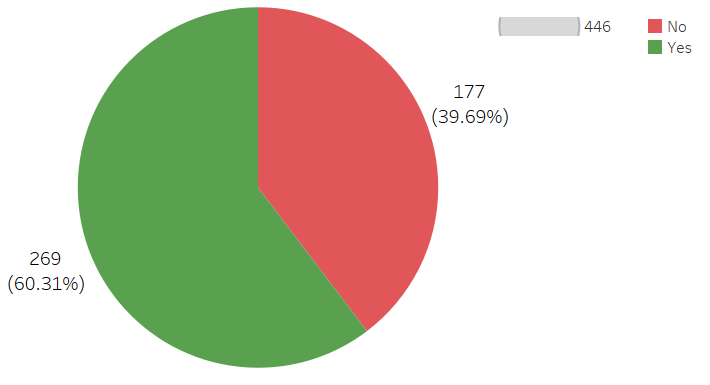
\includegraphics[width=0.8\textwidth]{immotionUsage}
    \caption{The Sum of Number of Records and Percentage of Total Number of Records for question ``\textit{Would you use the Immotion game for warm up?}''}
    \label{fig:immotionUsage}
\end{figure}\\
The pie chart in \ref{fig:immotionUsage} shows the number and percentage of respondents that would use the prototype game for warming up, and the number and percentage of the respondents who would not use the prototype game for warming up. From the information shown in this pie chart the green area resembles those who would use the Immotion game for warming up n = 269 (60.31\%) while the red resembles those who would not use it n = 177 (39.69\%). This question was asked from all the respondents (n = 446) regardless of their warm up preferences. From \ref{fig:immotionUsage} we conclude that the general acceptance of our gamified system is positive.\\ If we assess the respondents age compared to the Immotion game usage, we observe that the game is generally accepted by the respondents between age 22 and 37 years old. Negative responses concerning the warm up game usage are received from the respondents who were older than 38 years, presented in \ref{fig:UsageAge}.\\
Next, the acceptance of the Immotion warm up game regarding respondents' preferences towards warm up before a physical activity is depicted in \ref{fig:usage}. Out of n = 195 respondents who reported not warming up before sports activities n = 124 (63.58\%) would use the Immotion game for warming up. On the other hand, out of n = 251 respondents who reported always warming up before sports activities, n = 145 (57.76\%) would use the Immotion game for warming up.We observe that the general acceptance of the game is relatively high in both categories of respondents. However, respondents falling into category of athletes who do not warm up regularly gave more positive answers compared to the athletes who warm up regularly. This might imply that our gamified system is more appealing to respondents who do not engage in warm up routines often, and hence, could motivate them to warm up more regularly, or at least, more than they do currently. Also, high acceptance of the warm up game in the category of athletes who warm up regularly also tells us that those athletes, even though reported having well established warm up routines, would possibly switch to our solution if they are presented with the option to do so.\\
\begin{figure}[h]
    \centering
    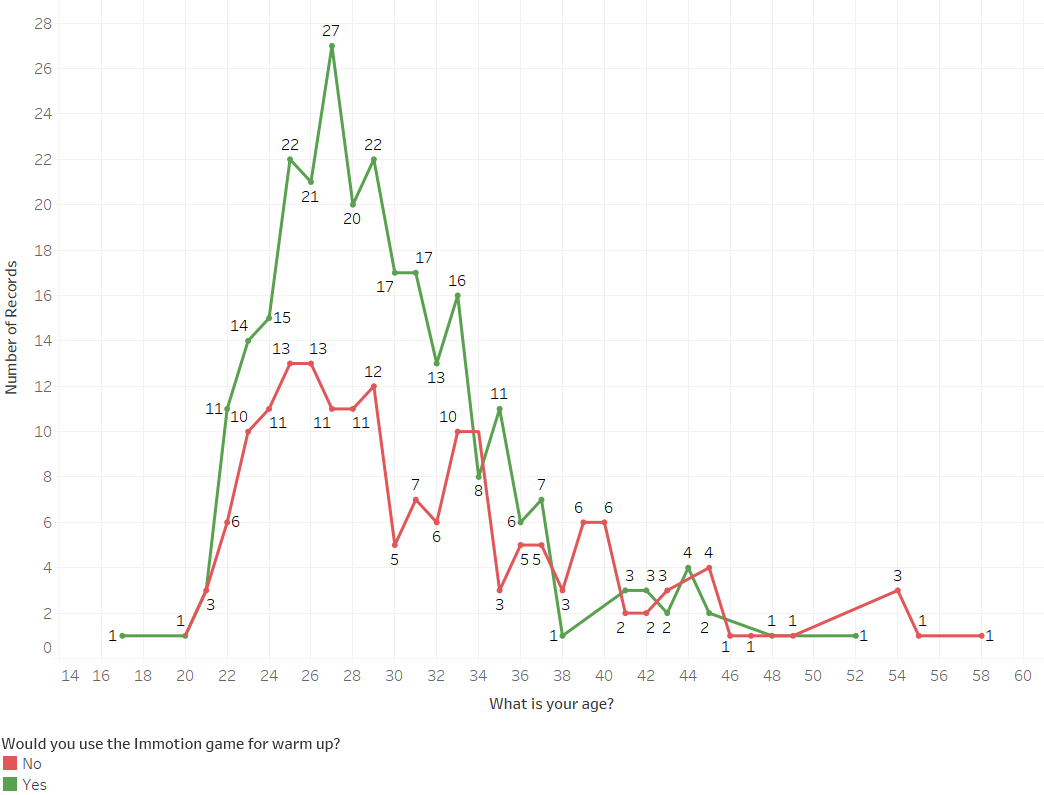
\includegraphics[width=0.8\textwidth]{UsageAge}
    \caption{The trend of sum of Number of Records for question ``\textit{What is your age?}''. Color shows details about responses to the question ``\textit{Would you use the Immotion game for warm up?}''}
    \label{fig:UsageAge}
\end{figure}
\begin{figure}[h]
    \centering
    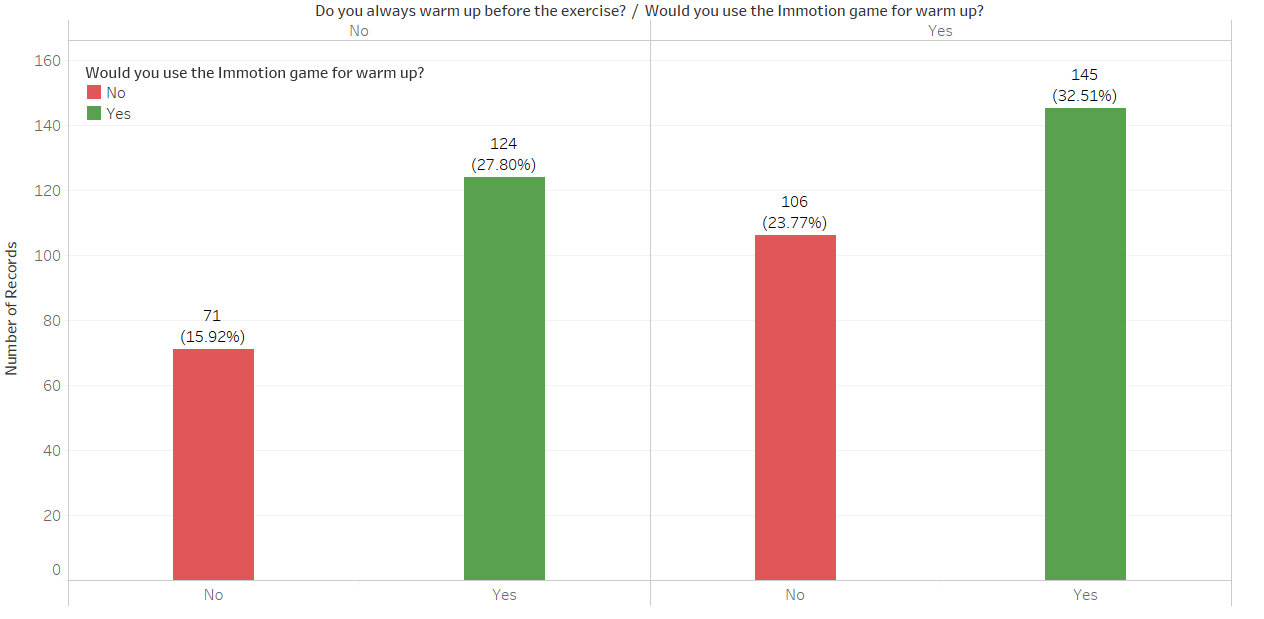
\includegraphics[width=0.9\textwidth]{usage}
    \caption{Sum of Number of Records for the question ``\textit{Would you use the Immotion game for warm up?}'' broken down by responses for question ``\textit{Do you always warm up before the exercise?}''. Color shows details about question ``\textit{Would you use the Immotion game for warm up?}''}
    \label{fig:usage}
\end{figure}\\
Since the player of the Immotion game is instructed when and what sort of movements to preform, we were interested in acceptance of the game among those respondents who prefer and do not prefer warming up when given instructions, shown in \ref{fig:warmupusage}.
\begin{figure}[h]
    \centering
    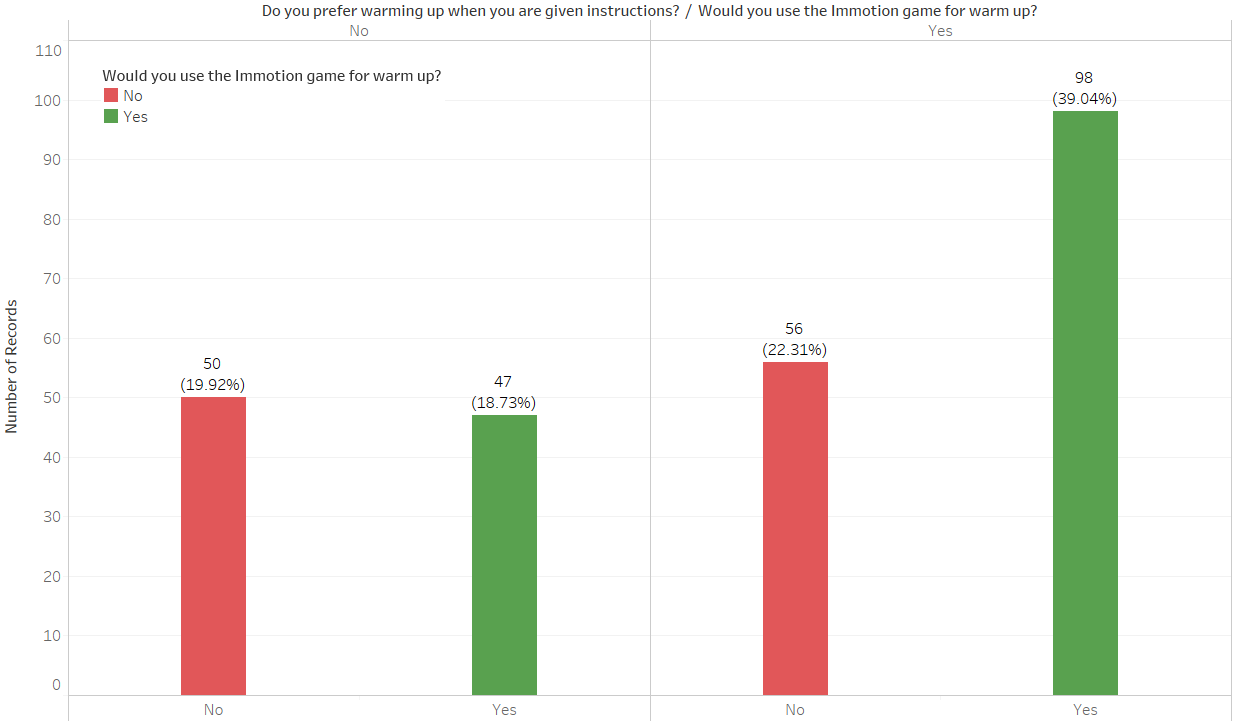
\includegraphics[width=\textwidth]{warmupusage}
    \caption{Sum of Number of Records for the question ``\textit{Would you use the Immotion game for warm up?}'' broken down by responses for the question ``\textit{Do you prefer warming up when you are given instructions?}''. Color shows details about the question ``\textit{Would you use the Immotion game for warm up?. }''}
    \label{fig:warmupusage}
\end{figure}\\
Out of n = 251 respondents who reported warming up regularly before sports activity, n = 97 stated not preferring having given instruction during the warm up exercises and n = 144 respondents stated that they prefer warming up when given instruction. From figure in \ref{fig:warmupusage}, we observe that out of all the respondents who do not like warming up when given insrtuctions, n = 50 respondents stated that they would not use the Immotion warm up game, while n = 47 respondents stated that they would use it. Contrarily, among respondents who prefer having instructions during warm up exercises, n = 56 stated that they would not use the warm up game, while n = 98 respondents reported that they would use it. From these responses, we see that the acceptance of the warm up game is much higher among those respondents who prefer warming up when given instruction and conclude that our gamified solution is more appealing for individuals who prefer warming up when given instructions. This also suggests that the warm up guidance and instructions that aree offered by our solution, could hypothetically influence individuals to engage in warm up routines more regularly.\\ Lastly, we analyze the warm up game acceptance broken down by respondents' preferences toward warming up alone, with a friend or in a group.\\\\
In \ref{fig:wuAloneUsage}, the respondents' answers are first sliced into categories based on the fact that they do or do not warm up before sports activities, and then broken down in subcategories based on their preferences toward warming up alone, with a friend or in a group.
\begin{figure}[h]
    \centering
    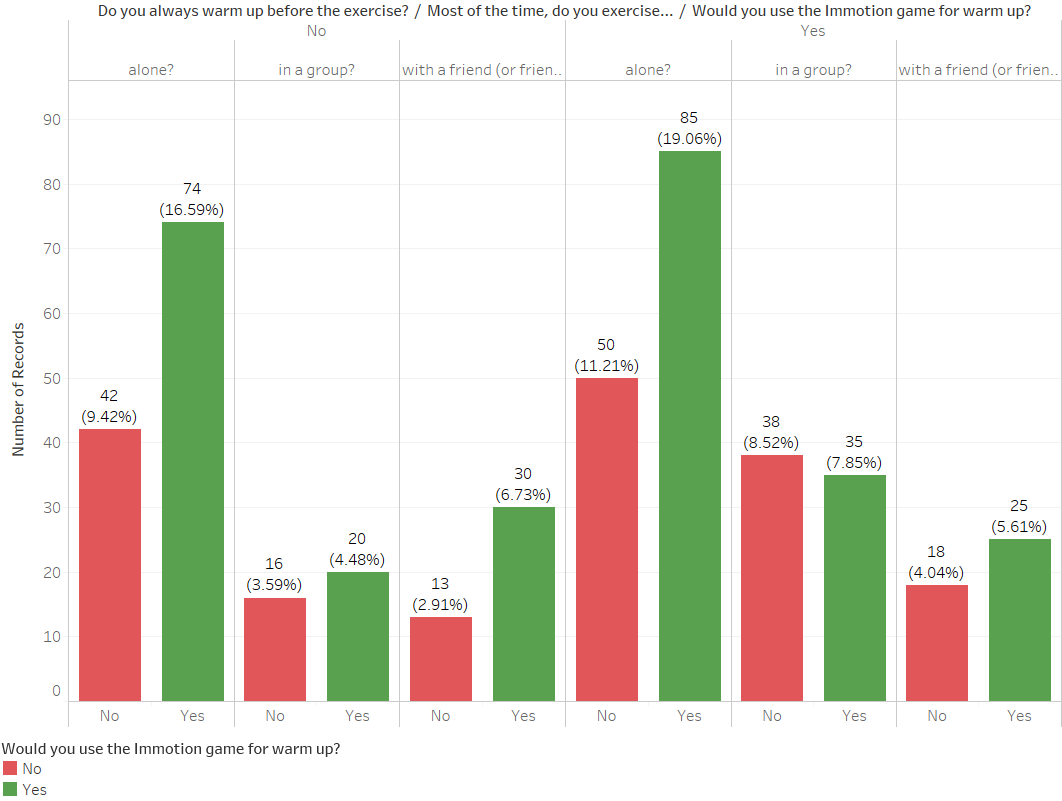
\includegraphics[width=0.75\textwidth]{wuAloneUsage}
    \caption{Sum of Number of Records for respondents' answers to ``\textit{Would you use the Immotion game for warm up?}'' broken down answers to ``\textit{Do you always warm up before the exercise?}'' and ``\textit{Most of the time, do you exercise alone, in a group or with a friend}''. Color shows details about answers to ``\textit{Would you use the Immotion game for warm up?}''}
    \label{fig:wuAloneUsage}
\end{figure}\\
We observe that the general acceptance of the warm up game is high in each subcategory (alone, with a friend, in a group) of respondents. The highest acceptance is among those athletes who prefer exercising alone (regardless of they warm up or not). The only subcategory where the disapproval of the gamified approach was higher than its acceptance, was among those respondents who warm up regularly and prefer exercises that are carried out in a group. We believe that the reason for this is the fact that the Immotion game, as shown in the video to the respondents, is a single player game which instructs the player to perform a set of general warm up movements. Respondents who engage in group (team) sports might not feel useful to spend time on general warm up exercises if the sport they engage in require specific movements. Furthermore, in exercises that are carried out in a group, it might not be time efficient to wait for every team member to complete the warm up routine using the proposed warm up game. That is, the proposed solution is not practical for the use case where athletes engage in group sports or exercises. This information, nevertheless, suggests that the target group for the Immotion warm up game should be individuals who prefer exercising alone or with a friend regardless if they warm up before sports activities or not.\\\\\\If we compare respondents' reasons for not warming up with respondents' general acceptance of the Immotion warm up game showed in figure \ref{fig:ReasonsWouldUse}, we observe that the game is generally accepted positively among all the respondents regardless the reasons they pointed out for not warming up.
\begin{figure}[h]
    \centering
    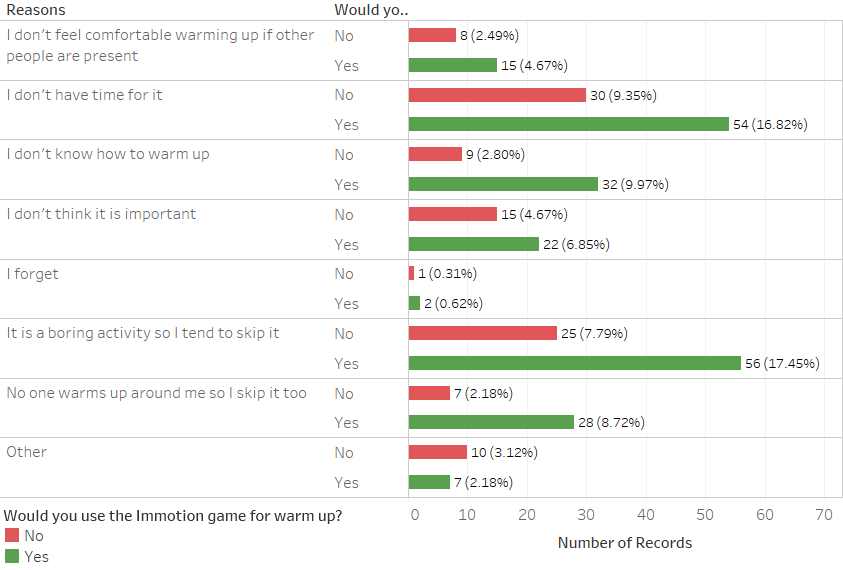
\includegraphics[width=0.9\textwidth]{ReasonsWouldUse}
    \caption{Sum of Number of Records for question ``\textit{Would you use the Immotion game for warm up?}'' broken down by respondents' reasons for not warming up. Color shows details about respondents' answers to the question ``\textit{Would you use the Immotion game for warm up?}''}
    \label{fig:ReasonsWouldUse}
\end{figure}\\
Lastly, when we slice the results based on respondents' gender, showed in \ref{fig:ReasonsWouldUseMakeFemale} , the result are similar to those depicted in \ref{fig:ReasonsWouldUse}. Overall, our gamified solution is positively accepted among all categories of respondents.\\ 
\begin{figure}[h]
    \centering
    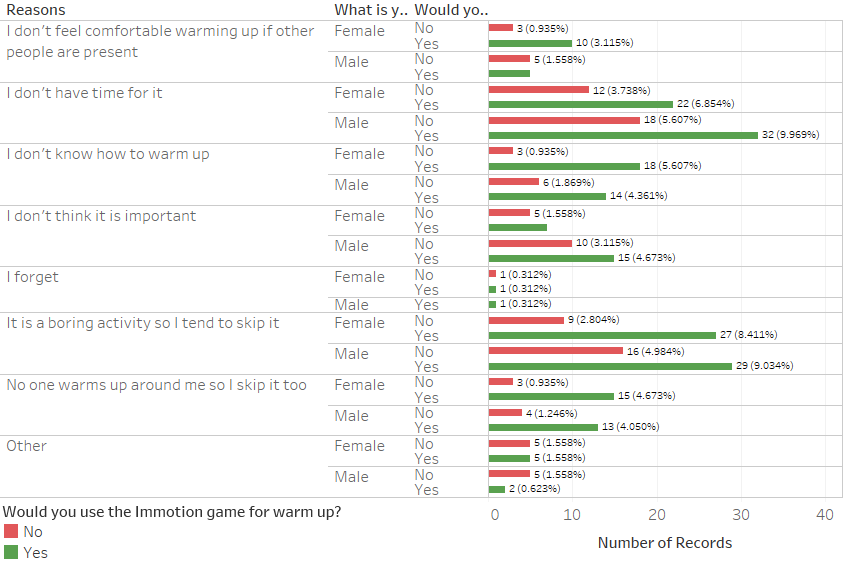
\includegraphics[width=\textwidth]{ReasonsWouldUseMakeFemale}
    \caption{Sum of Number of Records for question ``\textit{Would you use the Immotion game for warm up?}'' broken down by respondents' reasons for not warming up and respondents' gender. Color shows details about ``\textit{Would you use the Immotion game for warm up?}''}
    \label{fig:ReasonsWouldUseMakeFemale}
\end{figure}\\
To assess respondents' attitude towards the Immotion warm up game showed in the video, the respondents (n = 446) were asked to give their preferences regarding the following statements:
\begin{itemize}
\item ``\textit{I would rather use standard warm up routines instead of gamified warm up.}''
\item ``\textit{This approach (showed in the video) can increase the duration of my warm ups.}''
\item ``\textit{This approach (showed in the video) can increase the quality of my warm ups.}''
\item ``\textit{This approach (showed in the video) can make warm up more enjoyable for me.}''
\item ``\textit{This approach (showed in the video) can never work in practice for me.}''
\item ``\textit{This approach (showed in the video) could motivate me to warm up more regularly.}''
\end{itemize}
For each question, respondents could choose among five categories: Strongly Disagree, Disagree, Neutral, Agree and Strongly agree. Each category is assigned a score from 1 (Strongly Disagree) to 5 (Strongly Agree). Figure in \ref{fig:LS2} shows the Likert scale score for the previous statements sliced by respondents' preferences towards warming up before sports activities.\\
As in Likert scale presented in figure \ref{fig:LS1}, for each question we assign a range of values that show how the survey responses are spread by available categories and a general feeling whether they are positive or negative. Based on the available categories and their total scores, we specify the dividing line and check how many responses are below and above it. Each individual line shows a different starting point for each answer. The overall score (or the number of responses) for all the question is the same, since these questions were mandatory and all respondents answered it (n = 446). The width of each individual category depends on the number of records that are in that category over the total number of responses for the entire bar (that particular question). Lastly, we add the overall Likert scale score (LSS) depicted as a white circle in each bar which shows the summary for each individual question.  
From \ref{fig:LS2}, we observe that respondents who reported warming up regularly would rather use standard warm up routines instead gamified warm up solutions, like the presented Immotion warm up game (LSS = 3.59). On the other hand, respondents who do not warm up regularly mostly disagreed with the statements (``\textit{I would rather use standard warm up routines instead of gamified warm up.}'') or gave a neutral answer (LSS = 2.95). To be precise, n = 15 respondents strongly disagreed, n = 53 disagreed and n = 70 gave neutral answer out of n = 195 who reported not warming up before sports activity.\\ 
\begin{figure}[h]
    \centering
    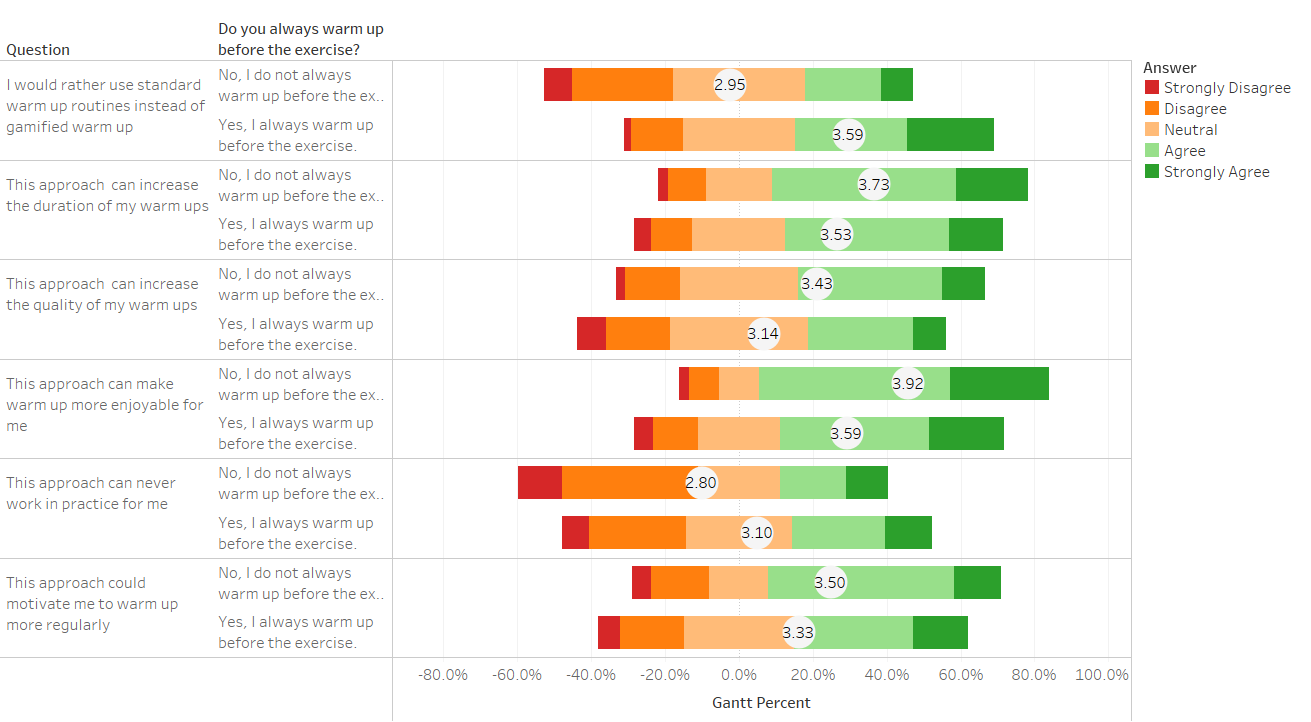
\includegraphics[width=\textwidth]{LS2}
    \caption{Gantt Percentage and the average score for question ``\textit{Do you always warm up before the exercise?}'' broken down by statements regarding the Immotion warm up game.}
    \label{fig:LS2}
\end{figure}\\ 
This suggests that most respondents falling into this category would likely use our gamified solutions as part of their work out (sports) routines. Regarding the second (``\textit{This approach (showed in the video) can increase the duration of my warm ups.}'') , third (``\textit{This approach (showed in the video) can increase the quality of my warm ups.}'') and sixth (``\textit{This approach (showed in the video) could motivate me to warm up more regularly}'') statement, both categories of respondents gave generally positive answers. However, respondents who warm up regularly gave more neutral answers (n = 63, n = 94 and n = 75 out of n = 251) which indicates their uncertainty about the possible positive effects this gamified solutions can have on the duration and the quality of the warm up procedure.  Similarly, in the fourth statement (``\textit{This approach (showed in the video) can make warm up more enjoyable for me.}''), responses given by both category of respondents were generally positive (LSS = 3.92, LSS = 3.59). This was, also, the statement that had the highest acceptance among respondents who do not warm up regularly. Overall, the results suggest that both categories see the gamified approach as a way of making the warm up routine more enjoyable and satisfying. The fifth statement (``\textit{This approach (showed in the video) can never work in practice for me.}'') received lover score (i.e. negative answers) from all the respondents. This corresponds to the previous results and suggests that respondents would presumably include this approach in their exercise routine if presented with the option.\\\\
If we slice the results by respondents' preferences towards exercising alone, with a friend or in a group, we observe that the respondents in all categories generally think that this gamified solution can increase the quality and the duration of their warm up routines and further make it more enjoyable, presented in \ref{fig:LS3}.\\
\begin{figure}[h]
    \centering
    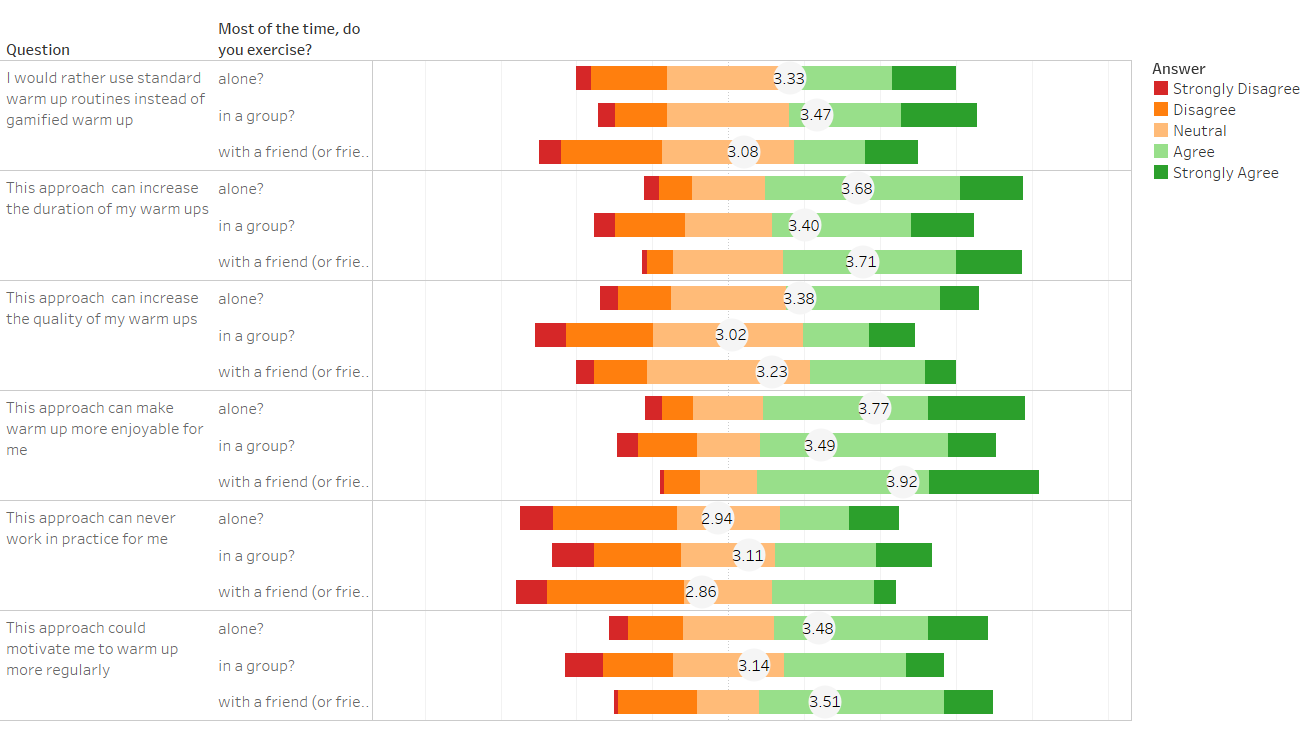
\includegraphics[width=\textwidth]{LS3}
    \caption{Gantt Percentage and the average score for question regarding respondents' preferences to warm up alone, in a group or with a friend broken down by statements regarding the Immotion warm up game.}
    \label{fig:LS3}
\end{figure}\\ 
Moreover, the possible positive affect that this approach can have on the consistency of the warm up sessions was received also well. The lowest scores were given by respondents who prefer exercises that are carried out in a group. In summary, taking into account the results depicted in \ref{fig:LS2} and \ref{fig:LS3}, our warm up game received positive acceptance from all the respondents, suggesting that it can hypothetically stand as a solution to increase the proportion of athletes who engage in warm up routines before every exercise or sports activity.\\ Lastly, all respondents were asked to leave their comments regarding the features they liked or disliked about the presented prototype warm up game, as well as to leave recommendations in case they have any. These questions were optional and not all the respondents actually responded. For all answered questions, we grouped the answers based on textual occurrences of specific keywords and on textual occurrences of keywords with the same semantic meaning.\\ In \ref{fig:1_mostImportantFeatures} we present the summary of responses regarding question ``\textit{What do you think are the most important features of this warm up game that would make you use it?}''\\\\ \\ \\
From \ref{fig:1_mostImportantFeatures} we observe that most of the respondents see the game as a fun, entertaining and enjoyable way for engaging in the warm up routine; a ``\textit{very new and creative idea to warm up}''.
\begin{figure}[h]
    \centering
    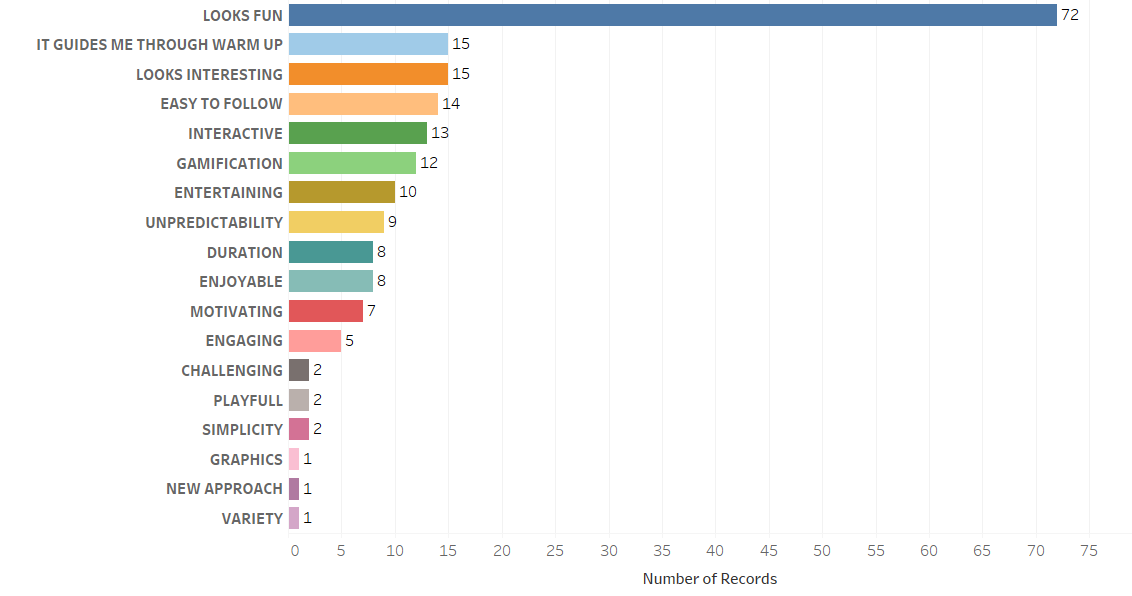
\includegraphics[width=\textwidth]{1_mostImportantFeatures}
    \caption{Aggregated answers for question: ``\textit{What do you think are the most important features of this warm up game that would make you use it?}''}
    \label{fig:1_mostImportantFeatures}
\end{figure}\\ According to the respondents, this warm up game would be the most useful ``\textit{for people that do not warm up or do not know how to warm up}''. This statement aligns with our assumption also. We believe that athletes who rarely or never warm up, as well as athletes who do not know how to perform a warm up routine would benefit from the presented gamified solution for warm up the most. Next, the respondents appreciate the guidance in the game, in a sense that they are instructed to which movements to perform through avoiding obstacles and collecting points:
\begin{itemize}
\item ``\textit{Very simple direction on what to do, once you get the mechanic of what the game is trying to get you to do you don't really have to think much about the varying motions asked of you, you're just trying to hit the orbs by moving your body as necessary.}''
\end{itemize} 
Moreover, they enjoyed the interactive element the game provides through the Kinect sensor, the gamification elements (coins) placed in game scenes and that it is made easy to follow. The obstacles and coins are situated in a way that is easy to understand which movement is required to perform in order to avoid the obstacle or collect more points and, thus, finish the game successfully:
\begin{itemize}
\item ``\textit{The game makes me unconsciously do a proper warm up without me thinking about the procedure and the exercises a lot.}''
\item ``\textit{Performed motions are changing often, definitely more interesting than 30 jumping jacks.}''
\end{itemize} 
Also, some of the respondents appreciate the short duration of the game because it can easily fit in their work out routine. In addition, they point out how this approach could motivate them to start their work out session with warm up and potentially influence the duration of the warm up exercise too. They attribute this to the gamification of the warm up routine and the immersive nature of the game that acts as a distraction, in a sense that, it engages the user and shifts users' focus from a tiresome warm up activity:  
\begin{itemize}
\item ``\textit{It's immersive - it would feel like a game and not a boring warm up routine.}''
\item ``\textit{Engaged without realizing.}''
\item ``\textit{It would increase the duration of my warm up - time passes faster when you are distracted by a video.}''
\end{itemize} 
Furthermore, the short and fixed duration of the game seems to be appealing to the respondents as well. By knowing exactly how long the warm up session will last, they believe that their work our session could be planned better.\\
In order to gain insight into elements of the game the respondents dislike the most, we asked them to point out the features, elements and main aspects of the game they would change or remove completely. These answers gave us more information about respondents' attitudes towards the presented warm up game and their stand about gamified solutions of exercises in general. Based on these answers and suggestions, we added new features and modified exiting ones, in order to have a gamified solution for warm up that fits respondents', and presumably future users', needs the most. Our goal is to offers a solution that can be used before every exercise and sports activity, and having elements and features users expect and desire the most, will make the game more appealing and, thus, more regularly used.
Figure in \ref{fig:2_whatDoYouDislike} shows the summary of responses regarding question ``\textit{What do you dislike about this warm up game with regard to the general idea (using game to motivate users to warm up more regularly)?}''
One of the interesting aspects that was captured during this survey is the main reason why respondents would not use the game. From the results in \ref{fig:2_whatDoYouDislike} we notice that most of the respondents pointed out the hardware (i.e. Kinect sensor, projector and large screens) and its price as the primary argument for not using the game. Surprisingly, from the video that was shown, the respondents assumed that in order to use the game, one must acquire all the necessary hardware and use the game at home before the sports activity:
\begin{itemize}
\item ``\textit{It's too impractical. I can't find a dark room with a projector before I play football or cricket.}''
\item ``\textit{No way would I warm up in one location (living room) before going to exercise.}''
\item ``\textit{Jumping disturbs the neighbors (next door and downstairs) when living in an apartment; prefer warm up outside}''
\end{itemize} 
Taking this into account, the negative bias is acceptable. However, as mentioned before, the game is intended to be used in gyms, fitness and sports centers, and it is not designed to be a solution for home work outs and exercises.
\begin{figure}[h]
    \centering
    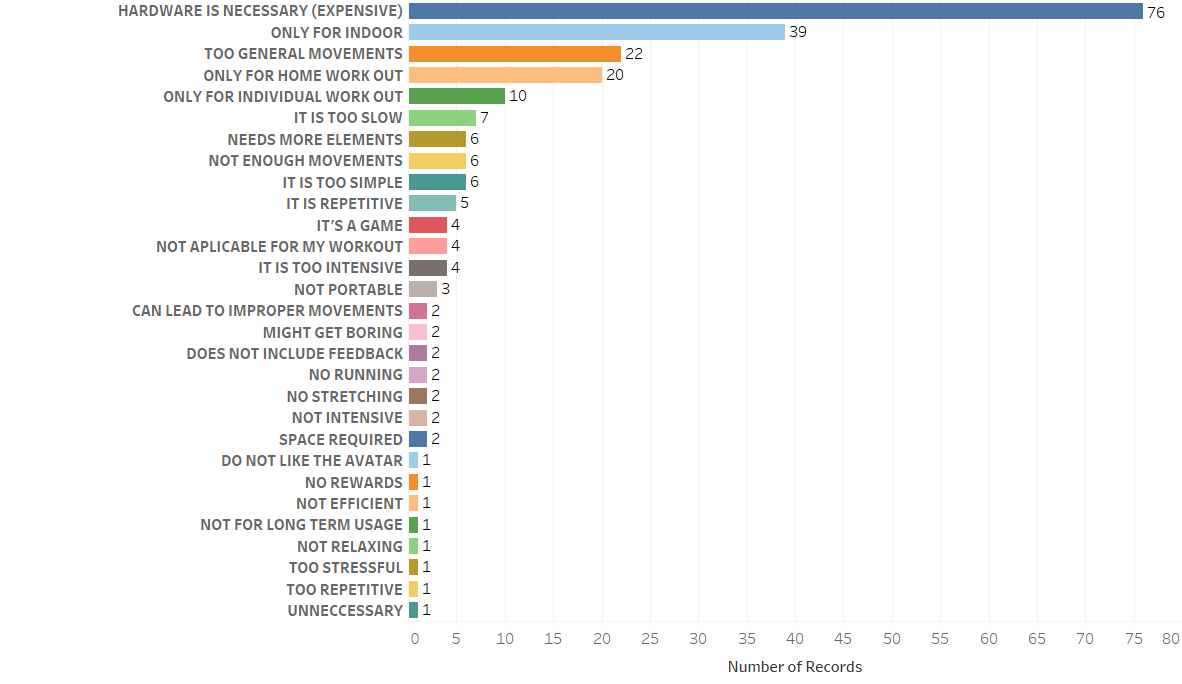
\includegraphics[width=\textwidth]{2_whatDoYouDislike}
    \caption{Aggregated answers for question: ``\textit{What do you dislike about this warm up game with regard to the general idea (using game to motivate users to warm up more regularly)?}''}
    \label{fig:2_whatDoYouDislike}
\end{figure}\\
Since games  work out that are intended to be used at home already exist on the market, our goal is to completely focus on the warm up gamified solution as a preparatory activity before sports sessions and to make it available and usable in places where individuals come to engage in some sort of sports activity. That way, we hypothesize, our approach will be more likely utilized, compared to home work out solutions. In addition to this, respondents who prefer sports and work out exercises outdoor, mostly disliked the fact that the game is intended to be used indoors without any option to be installed and used in open space. This was the second most argued reason for not using the presented game:
\begin{itemize}
\item ``\textit{The issue is that the game has to be setup where I do my sport, which is probably not going to happen (forest)}''
\item ``\textit{You need to do it in a room with a screen and a device, this is a strong constraint if you want to practice sport outdoors}''
\item ``\textit{Most of my warm ups take place outside, and so it may not work outdoors very easily}''
\end{itemize}
They propose having a portable version (mobile application) of the game that can be used without any space or hardware constraints. These recommendation will be further assessed later in this chapter. Furthermore, the respondents pointed out that only few movements (exercises) are required in the game which makes it one-dimensional, neglecting the warm up for arms and upper body:
\begin{itemize}
\item ``\textit{Very limited range of motion, hard to imagine it would capture all required muscle groups one should normally warm up.}''
\end{itemize}
We assume that the reason they find the movements too general and repetitive is because only few exercises and movements were included in the prototype that was presented to them. The prototype had 7 segments and only 4 segments contained obstacles with coins. In the prototype game, the obstacles are avoided and the coins collected using jumps and right and left movements, depending on the position of the game elements. Introducing only limited number of segments and requiring only few movements were determined to be sufficient to present our idea of gamified warm up and assess its general acceptance. For the second release of the warm up game, based on the respondent' answers regarding most common movements and exercises they reported performing during warming up (presented in \ref{fig:5_describeWURoutine}), we extend the number of movements required to carry out in order to successfully finish the game. We believe that we captured and implemented the most common exercises and movements reported by the respondents that are, first, detectable with high accuracy using only one Kinect device and, second, accomplished easily without no prior exercise knowledge or experience. Moreover, we decide to discard and not implement movements that are reported by most of the respondents but require additional equipment in order to be performed, like pull-ups, rowing and rope jumping. 
Next, the respondents mentioned the lack of group (or multiplayer) exercises using the game. Since some of the respondents often engage in group sports, they would expect that the game also includes a version where they can compete with someone while warming up, or just warm up using the game together with the group they exercise with:
\begin{itemize}
\item ``\textit{You could design the game so that it is competitive. You could compete with other players for a high score, and this could become a group activity and become a part of exercise routines. This way, it would also become easier for you to drag someone who doesn't exercise regularly to start doing so.}''
\end{itemize}
This requirement is often mentioned by the respondents. According to the respondents, this feature is necessary for group sports sessions. Introducing this feature could make the game more enjoyable and boost the competitive aspect of the game:
\begin{itemize}
\item ``\textit{It's not practical if you exercise in groups. In this case everyone would need their own screen, which seems like too much of a hassle just to warm up.}''
\end{itemize}
The simplicity of the scenery, used avatar and lack of diversified game elements was also brought up. According to the users, the absence of these elements can potentially make the game monotonous and uninteresting for them after a while. If the game is lacking captivating visuals and scenery, compelling challenges and intriguing story line, users will stop using it after the initial incitement for the game ceases. Taking this into account, we introduce new segments with elements that make the game more appealing and the challenges more attractive. We increase the number of segments from 7 to 20 and completely change the scenery previously presented in the prototype game. Regarding types of exercises performed in the game, many respondents expressed their concerns that stretching exercises are not included in the required movements: 
\begin{itemize}
\item ``\textit{Depending on the efficacy, I would want to incorporate stretching as part of the routine. Even if it was doing some motion detection for active stretching in a direction to pop balloons or something.}''
\item ``\textit{… does not stretch ligaments for my sports (body building)}''
\end{itemize}
Since stretching is part of most respondents' warm up routine, they expect that the game also contains movements and exercises of this type. They propose having movements that focus on whole body stretching, stating it helps them to prepare more for the subsequent physical activity. This statement is surprising since research, as previously discussed,  has never found stretching warm ups to have any benefits in preparing our body for strenuous activity or injury prevention \cite{pereles2012large}. Thus, we choose not to incorporate stretching exercises as required movements in the second release of the game. However, at the end of the game, athletes will be informed about the duration of stretching exercises assumed to be the most beneficial for the subsequent activity. Lastly, the respondents pointed out that the intense focus on the screen could potentially lead to improper execution of the body movement and thus, lead to injuries:
\begin{itemize}
\item ``\textit{When you're not focusing on your movements, you are at a higher risk for injury. Additionally, muscles are more responsive when you're consciously engaging them.}''
\item ``\textit{I worry that I would not use proper technique when playing the game and therefore not successfully warming up.}''
\end{itemize}
They suggest monitoring the correctness of the movements performed by the users and, in case of incorrect ones, inform them in a way it does not affects their performance in the game as a form of a feedback:
\begin{itemize}
\item ``\textit{I think having an interactive screen that takes you through a proper warm up and can educate you on how to properly warm up each muscle and what each movement is warming up would be a great idea.}''
\end{itemize}
Some of the respondents argue that the game requires too general movements and exercises that are too generic and not applicable for the sports they engage in. These athletes usually perform specific warm up exercises that are either too complex to be captured with high precision by the Kinect sensor, or are executed in environment not suited and intended for our gamified solution (e.g. swimming, climbing). In summary, we would like to focus on more general exercises that are simplistic, presumably known by the athletes and can be captured with high accuracy using only one Kinect sensor. Moreover, we want to avoid stretching exercises because they do not provide protection from muscle soreness, they do not seem to contribute to the reduction in the risk of injury and, lastly, there exists insufficient research to support its effectiveness on sporting performance.\\  Figure in \ref{fig:3_featuresToBeUsedRegularly} shows the summary of responses regarding question ``\textit{In your opinion, what features does this game have to possess in order to be used on a regular basis?}''.\\
\begin{figure}[h]
    \centering
    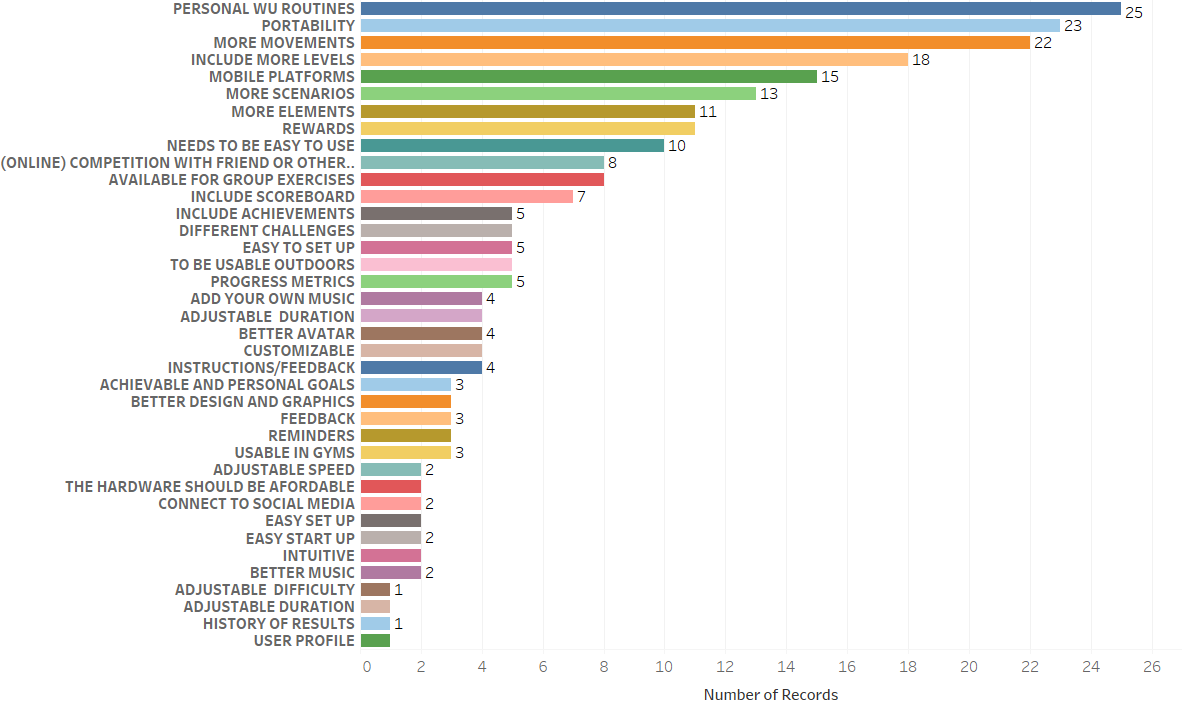
\includegraphics[width=\textwidth]{3_featuresToBeUsedRegularly}
    \caption{Aggregated answers for question: ``\textit{In your opinion, what features does this game have to possess in order to be used on a regular basis?}''}
    \label{fig:3_featuresToBeUsedRegularly}
\end{figure}\\
With this question, our goal was to gain insight into possible features and elements the respondents would look forward to and benefit the most from, in a gamified solution like the presented prototype. Based on these answers, ideas and recommendations we modify our game in order to be more appealing to the future users. From \ref{fig:3_featuresToBeUsedRegularly} we observe that the most of the respondents would enjoy having a gamified solution that is tailored specifically to their needs. That is, the respondents would like to have the option to customize and personalize the warm up routines in the gamified system. According to the respondents, the warm up movements should be adapted to the sport of choice and should also change overtime to avoid the routine being too repetitive.\\
 Namely, the warm up routines should be sports specific, and not general as in the presented video:
\begin{itemize}
\item ``\textit{It would be great if the game had different types of warm ups based on two things:  type of sport activities, which I am about to start (e.g. running, cycling, etc.) and if I have some specific preconditions, like back pain.}''
\item ``\textit{… different levels (for amateurs and for more professionals), different warm ups for different sport activities (e.g. warm up for a run or warm up for a HIIT session)}''
\end{itemize}
Moreover, the game should also take into account any physical injury users have. That is, individuals should be in position to discard some of the movements in case they are not able to perform them. In addition, adjustable game setting are also high in demand. The respondents would rather enjoy having a game with adjustable game elements (segments and avatar), speed, duration and number and types of obstacles. That way, they would be in control of the movements that are needed to be performed, as well as, their intensity and speed. This requirement is actually tightly connected to the one previously mentioned. The respondents would prefer the most to be able to manage and manipulate all the game's features conforming them, by doing so, to their work out preferences. Portable (and mobile phone) version of the game, as in the previous question, is also pointed out by the respondents:
\begin{itemize}
\item ``\textit{As with team sports, location changes weekly so if this game was able to be moved with the team then this would help.}''
\end{itemize} 
Users who engage in sports outdoors or whose work out location changes often, would prefer having a mobile application that helps them warming up. Moreover, the respondents would rather enjoy a game that has more levels with different sceneries and difficulties. Each level, according to respondents, could be at different difficulty level, including new obstacles and, hence, require new movements in order to avoid those obstacles. This way, they believe, the game will stay enjoyable and captivating for a longer period of time:
\begin{itemize}
\item ``\textit{Interesting and achievable goals, something new all the time, new routes, obstacles, etc.}''
\item ``\textit{More movements and as time goes by, the speed of the obstacles you approach should be faster, different and finally a short cool down at the end like just walking for a minute.}''
\end{itemize}
Currently, only one level is available. We believe that introducing multiple levels is an option worth considering. However, we opted for the solution with diversified scenes and elements instead. Gamification elements like scoreboards, awards, achievements and progress metrics were also brought up by the respondents. %should add references to related work here!%
According to the answers, including these elements would make the game more engaging and satisfying. Next, some of them would gladly share their achievements on social media. Hence, connecting the game with social networking platforms would also influence some users to use our gamified solutions. Regarding game graphics and sounds, diversified scenes, being able to choose from multiple avatars and importing custom music playlist was mentioned by the respondents also. Multiplayer version of the game, where one can warm up or compete with someone, according to the respondents, would make the game more appealing and usable.\\ 
Lastly, we asked the respondents to leave comments and recommendations regarding the presented prototype warm up game. We wanted to gain insight into possible features and elements expected by the respondents which could be incorporated in the game. We acquired interesting suggestions and ideas from the respondents, some of which, are implemented in the second version of the game. Figure in \ref{fig:4_recommendations} shows the summary of responses regarding question ``\textit{Do you have any recommendations or suggestions regarding the game?}''\\
\begin{figure}[h]
    \centering
    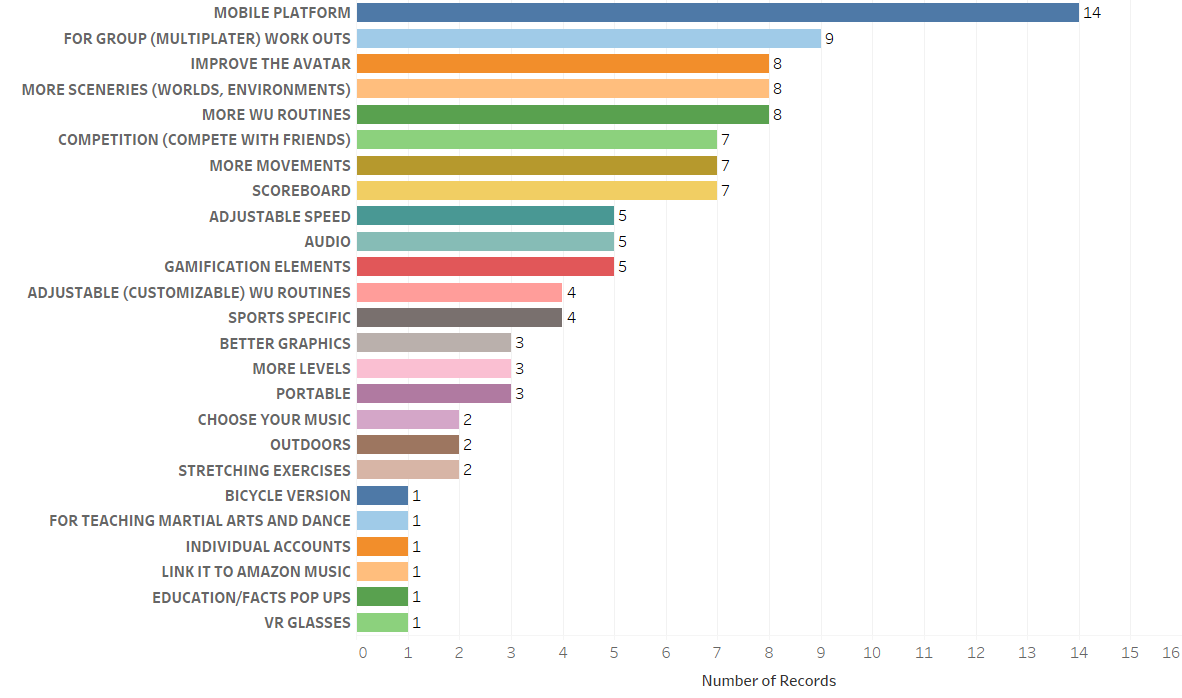
\includegraphics[width=\textwidth]{4_recommendations}
    \caption{Aggregated answers for question: ``\textit{Do you have any recommendations or suggestions regarding the game?}''}
    \label{fig:4_recommendations}
\end{figure}\\ 
From \ref{fig:4_recommendations} we notice that most of the respondents recommended designing and implementing a portable version of the game that is not constrained by any additional hardware currently required for game functioning.\\ \\ \\They suggest having a ``\textit{pocket version}'' the game that can ``\textit{easily be watched on a smartphone}'':
\begin{itemize}
\item ``\textit{Could be on an app form, everyone has a phone they can use; having arrows on the screen about which direction to use. Not as fun but just as effective.}''
\item ``\textit{Well, if the whole same thing can be done on mobile, this will be a great success.}''
\end{itemize}
Furthermore, a multiplayer (group) version of the game where users can compete with others seems to be a very appealing feature most of the respondents brought up: 
\begin{itemize}
\item ``\textit{… I actually think turning it into a competition would be cool where you have different players (and you can add your friends) and then see who completes the warm up with the most points (like Mario Kart or something similar)}''
\end{itemize}
We agree to this suggestion and hypothesize that by creating the option for competitions between athletes, our gamified system would provide users with a solid reason to keep returning to it and, in turn, help with creating a healthy habit of warming up before more strenuous exercises. By keeping track on athletes' performance on how many points have been collected during the warm up session, and also displaying these results in a form of scoreboard, our gamified solution could provide motivation to someone who might not be able to find it on its own.
Most of the respondents did not like the avatar that was used in the prototype version of the game. We expected this reaction since the avatar that has been used did not have humanoid features and was represented using simple lines (skeleton). However, it replicated correctly the user's movement which was our goal with the prototype version of the game: 
\begin{itemize}
\item ``\textit{Having a relatable character that does the workout.}''
\item ``\textit{Obviously it's a prototype, but it'd be better to see a real person or game character in place of a dummy.}''
\end{itemize}
Studies have also found that having avatars that are idealized version of our self can influence how much we enjoy the game and how immersed we become. They continue by saying that people also tend to ``unconsciously conform to the expectations of their avatar's appearances'' \cite{avatar}. Taking this into account, we replace the avatar in second release of the game and chose one that is more relatable and have a correct posture, as suggested by the respondents: 
\begin{itemize}
\item ``\textit{Maybe to think over different positively looking characters with healthy right-looking postures so that a trainee's body can subconsciously copy and remember it.}''
\end{itemize}
Even though many respondents suggested a version of the game with a customizable character or a version of a game with multiple characters one can choose from, the second release of the game contains only one avatar. We want to make the game easy to use and promptly to start. Having implemented the option with multiple and customizable character, we believe, would require more time for initial game start and, thus, increase the duration of the warm up routine altogether. We would not like for the users to spend more time designing more likable avatars than engaging in the warm up routine. This option is, however, very appealing and will be considered for future game releases. Apart from that, many respondents recommended having more movements and exercises one needs to perform in order to complete the game that can be, in the same time, personalized and customizable (sport specific), as discussed earlier.\\In the next section, a short summary of the survey results, together with the changes that will be included in the second release of the Immotion warm up game are presented. \pagebreak
\subsection{Survey Summary and Preliminary Design Implications}
To gain a first insight into acceptance of the Immotion warm up game we created an online survey. The goal of this survey was to explore general work out and warm up habits of the respondents and the general acceptance of our gamified solution for warm up. We hypothesize that gamified warm up solutions can make warm up routines more enjoyable and, thus, motivate individuals to warm up more regularly before physically more demanding exercises. Total number of n = 446 individuals participated in the survey, of which n = 204 (45.7\%) were female and n = 242 (54.3\%) male. The age of the respondents ranged from 17 to 58 with an average age of 30.16 years (SD = 6.49). When asked about their warm up preferences before a physical activity, n = 251 respondents (56.3\%) reported always warming up before physically more demanding exercises (or sports activities), whereas n = 195 (43.7\%) reported not warming up regularly before physically more demanding exercises (or sports activities). This category of respondents have been inquired about the reasons for avoiding warm up exercises before more strenuous physical activity. The results obtained, align with the ones acquired by Fradkin, et al. []. This further justifies the need for educational and motivational solutions, which are enjoyable and easy to carry out, with primary focus on the major muscle groups and benefits of warm up, in order to increase the proportion of athletes who engage in warm up routines before every exercise.\\In the last, third part, of the survey, the respondents were shown a short video with the prototype of the Immotion warm up game. In the prototype game, the players' movements were captured using one Kinect motion sensor and the game displayed on the wall using a projector. In order to complete the game successfully, and consequently warm up, the player was required to avoid obstacles and collect coins. Obstacles were avoided by performing general exercises like squats, jumps and movements to right or left. Total of n = 269 (60.31\%) respondents reported that would use the prototype Immotion game for warming up while n = 177 (39.69\%) would not use the prototype Immotion game for warming up. Out of n = 195 respondents who reported not warming up before sports activities n = 124 (63.58\%) would use the game for warming up. On the other hand, out of n = 251 respondents who reported always warming up before sports activities, n = 145 (57.76\%) would not use the game for warming up. We observe that the general acceptance of the game is positive in both categories of respondents, however respondents who do not warm up regularly would more likely use the proposed solution. Next, all the respondents were asked to give their preferences regarding specific statements we assessed would offer us more insight into respondents' attitudes towards gamification of warm up and our proposed solution. In summary, our warm up game received positive acceptance from all the respondents. However, the obtained results suggest that most respondents who do not warm up regularly would more likely use our gamified solutions as part of their work out (sports) routines compared to the category of respondents who reported warming up regularly, suggesting that it can hypothetically stand as a solution which can increase the proportion of athletes who engage in warm up routines before every exercise or sports activity. Moreover, the results imply that both categories of respondents see the presented gamified approach as a way of making the warm up routine more enjoyable and satisfying and that it could increase the quality as well as the duration of their warm up routines. Overall, the results obtained suggest that the respondents would include our gamified solution for warm up in their exercise routine if they are offered with this option.\\The respondents were further requested to give feedback regarding elements of the game they preferred the most and think a gamified solution like the presented one should possess. In addition they were also asked to point out the features, elements and main aspects of the game they would rather change or remove completely. These answers gave us more information about respondents' attitudes towards the presented warm up game. Based on these answers and suggestions, we added new features and modified exiting ones, in order to have a gamified solution for warm up that fits respondents', and presumably future users', needs the most. Since our goal is to offer a solution that can be used before every exercise and sports activity, having elements and features users expect and desire the most, we believe will make the game more appealing and, thus, more regularly used. The evaluation results from the first survey, as well as respondents' suggestions and recommendations were used to improve the Immotion game in order to be more enjoyable for the future usage.\\ Overall, the results that influenced design decisions for the second release can be generalized as follows:
\begin{enumerate}
\item Game design related
	\begin{enumerate}
		\item Avatar design\\
The respondents argued that the avatar used in the prototype version of the game is not relatable enough. We expected this reaction since the utilized model did not have humanoid features and was represented using simple lines. Taking this into account, we replace the avatar in second release of the game with a humanoid model that is more relatable and have a correct body posture, as suggested by the respondents.
\item Different game sceneries\\ 
According to the respondents, in the absence of the captivating visuals and sceneries, the game can become monotonous and uninteresting after a while. Thus, the scenery is redesigned completely to be visually more appealing and attractive. The game segments with empty walls and boxes that built up the game scenes are removed and the main character is placed in a jungle environment with ancient ruins and various creatures. 
\item Different obstacles\\
In the prototype of the game presented to the respondents, only one type of obstacle was placed in the game segments.  As expected, the respondents argued that the number and types of obstacles need to be increased in order to make the game more interesting and challenging. Hence, we introduce diversified elements that pose as obstacles to be avoided in the second release. We incorporate models of the remains of ancient buildings, old bridges, trees, trunks and different creatures.  
\item Multiple levels\\
The respondents would rather enjoy a game that has more game levels. Each level, according to respondents, could be at different difficulty, including new obstacles and, hence, require new movements in order to avoid those obstacles. We believe that introducing multiple levels is an option worth considering. However, we opted for the solution with diversified game segments and elements instead. The newly introduced obstacles and game elements are generated at random. Hence, each warm up session carried out with our gamified solution is different than the previous, in a sense that the order by which the game segments, and thus the obstacles, are presented to the user are random.  
\item Achievements and rewards\\
The prototype version of the game did not include any rewards or achievements. Including gamification elements like those, according to the respondents, would make the game more challenging and motivate them to take part in it more often. Achievements and awards can be tied to feedback because they are evaluative in nature. By using them, players can reflect on their performance which, consequently increases their perception of competence.  As a result, players' intrinsic motivation can be increased []. In the second release of our warm up game, a new reward system has been introduced. Based on the number of consecutive coin collections, if not hit by an obstacle, the player is awarded by certain amount of additional points. The full description of introduced reward system is detailed in Section XX. 
\item Scoreboard\\
In the second release of our gamified system, we introduce a scoreboard that displays the number of points the player collects. This gamification element is brought up by many respondents as a way of encouraging players to compete. As per various studies, the very presence of a scoreboard can often elicit the desire to play and the goal of advancing in the rankings can serve as a powerful motivator to continue []. 
\item Feedback and metrics\\
The respondents also suggested that the game should monitor the correctness of the movements performed by the users and, in case of incorrect ones, inform them in a way it does not affects their performance in the game. The feedback should, also include different metrics concerning users' energy and calorie expenditure as well as which muscle groups are used in certain movements during the game. Although this suggestion is interesting, we decide not to include direct feedback or metrics during the game. We believe that having all these metrics displayed during the game would be a distraction that will negatively impact the player's performance. Additionally, having only one motion sensor, the complete and correct mapping of the player's body and performed movement can be error prone. The only feedback the user receives during the game is in the form of rewards in case the required conditions are met. Out of the requested metrics, after the game has ended, we display the player's calorie expenditure, number of points reached and the current position on the scoreboard.  
The description and in depth overview of the second release of the warm up game is given in section XX.
	\end{enumerate}
\item Game features related
\begin{enumerate}
	\item Customizable game settings (Avatar, Obstacles, Speed, Duration)\\
The respondents would rather enjoy having a game with adjustable game elements (segments and avatar), speed, intensity and duration. That way, they argue, would be in control of the movements that are needed to be performed, as well as, their intensity and speed. That is, they would prefer the most to be able to manage and manipulate all the game's features conforming them, by doing so, to their work out preferences. Even though many respondents suggested a version of the game with a customizable avatar or a version of a game with multiple avatars one can choose from, the second release of the game contains only one. Moreover, we decided that the game segments will not be editable by the players. That is, players will not be in position to remove some of the game segments together with its obstacles. Our goal is to make the game easy to use and promptly to start. Having implemented the option with multiple or customizable avatars and game segments, we believe, would require more time for initial game start and, thus, increase the duration of the warm up routine altogether. The only adjustable game setting in the second release of the game is the duration. Based on the answers regarding most common warm up duration, we allow players to select their preferred warm up duration. The game speed, as in the original version, will increase gradually based on players' performance.  
\item Multiplayer option\\
Most respondents pointed out that the presented solution is not suitable for group (or multiplayer) exercises. Since some of the respondents often engage in group sports, they would expect that the game also includes a version where they can compete with someone while warming up, or just warm up using the game together with the group (or friend) they exercise with. We agree that introducing this feature could hypothetically engage more categories of athletes to warm up regularly, provide users with a solid reason to keep returning to it and, in turn, help with creating a healthy habit of warming up before more strenuous exercises. However, in the second release of the game, only single player option is available. In the survey, more than half of the respondents (n = 251) stated that they prefer exercising alone (56.3\%), n = 86 (19.3\%) with a friend (or friends) and n = 109 in a group (24.4\%). Thus, as being the majority, we decide to adapt this game feature to those athletes who prefer individual work out (sports) sessions and consider the multiplayer version for one of the subsequent game releases. 
\end{enumerate}
\item Required movements related
\begin{enumerate}
\item Increase required movements\\
The respondents pointed out that only few movements (exercises) are required in the game which makes it one-dimensional, neglecting the warm up for arms und upper body. The prototype solution that was presented to the respondents had 7 segments and only 4 contained obstacles and coins which needed to be collected using jumps or right and left movements, depending on the position of the game elements. Introducing only limited number of segments and requiring only few movements were determined to be sufficient to present our idea of gamified warm up and assess its general acceptance. For the second release of the warm up game with increased number of game segments, based on the respondents' answers regarding most common movements and exercises they reported performing during warming up (Figure 10), we introduce new movements required to carry out in order to collect points and avoid obstacles. We believe that we captured and implemented the most common exercises and movements reported by the respondents that are, first, detectable with high accuracy using only one Kinect device and, second, accomplished easily without no prior exercise knowledge or experience. Moreover, the second release will not require movements that are reported by most of the respondents but require additional equipment in order to be performed, like pull-ups, rowing and rope jumping.
\item Sports specific exercises\\
Some of the respondents argued that the prototype game requires too general movements and not targeting muscle groups that are relevant for the sports they engage in. These athletes usually perform specific warm up exercises that require prior knowledge of the exercise in order to be executed correctly, are too complex to be captured with high precision using only one Kinect sensor, or are performed in settings not suited and intended for our gamified solution (e.g. swimming, climbing).  Taking into account the responses regarding types of movements the responses usually perform in order to warm up (Figure 10), and since only limited number of respondents actually engage in specific warm up routines, in the second release of our gamified system we only focus on exercises that are simplistic, presumably known by the athletes and can be captured with high accuracy using only one Kinect sensor.
\item Include stretching exercises\\
Since stretching is part of most respondents' warm up routine, they also expect that the presented solution contains movements and exercises of this type. They propose having movements that focus on the whole body stretching, stating it helps them to prepare more for the subsequent physical activity. However, as previously pointed out, studies have never found stretching warmups to have any benefits in preparing our body for strenuous activity or injury prevention []. Thus, the second release will not incorporate stretching exercises as required movements. \\In the second stage, based on the feedback and reactions received from the respondents in the first stage, we complete the implementation of the second release of our gamified system and conduct a user study in a local fitness center. Our goal is to assess whether athletes would use our gamified solution to warm up and if it can motivate them to engage in warm up exercises more regularly.
\end{enumerate}
\end{enumerate}



